%%%%%%%% ICML 2026 SUBMISSION %%%%%%%%%%%%%%%%%
\documentclass{article}

\usepackage{microtype}
\usepackage{graphicx}
\usepackage{subcaption}
\usepackage{booktabs}
\usepackage{hyperref}
\newcommand{\theHalgorithm}{\arabic{algorithm}}
\usepackage{icml2026}

\usepackage{amsmath}
\usepackage{amssymb}
\usepackage{mathtools}
\usepackage{amsthm}
\usepackage[capitalize,noabbrev]{cleveref}

\theoremstyle{plain}
\newtheorem{theorem}{Theorem}[section]
\newtheorem{proposition}[theorem]{Proposition}
\newtheorem{lemma}[theorem]{Lemma}
\newtheorem{corollary}[theorem]{Corollary}
\theoremstyle{remark}
\newtheorem{remark}[theorem]{Remark}

\newcommand{\simplex}{\Delta^{D-1}}
\newcommand{\yh}{\hat y}
\newcommand{\E}{\mathbb{E}}
\renewcommand{\Pr}{\mathbb{P}}
\newcommand{\chisq}{\chi^2}
\newcommand{\Dir}{\mathrm{Dir}}

\icmltitlerunning{Which Geometry for Conformal Regions on the Simplex?}

\begin{document}

\twocolumn[
  \icmltitle{Which Geometry for Conformal Regions on the Simplex?\\
  Evaluating Coverage, Conditional Validity and Size for Compositional Outputs}

  \begin{icmlauthorlist}
    \icmlauthor{Anonymous Authors}{anon}
  \end{icmlauthorlist}
  \icmlaffiliation{anon}{Anonymous Institution}
  \icmlcorrespondingauthor{Anonymous Authors}{anonymous@example.com}
  \icmlkeywords{conformal prediction, compositional data, evaluation, conditional coverage}
  \vskip 0.3in
]

\printAffiliationsAndNotice{}

\begin{abstract}
Many predictors output a composition---a non-negative vector summing to one, such as a softmax or a topic-proportion vector---and users need to know whether the attached uncertainty is reliable.
Split conformal prediction gives marginal coverage for \emph{any} nonconformity score, so the choice of score (the ``geometry'' of the region on the simplex) is invisible to the usual coverage check and has to be judged by other criteria.
We study how to evaluate and choose that geometry.
(i)~We propose a protocol that reports coverage as a distribution over calibration sets (checked against the exact Beta law), conditional coverage over slices with a null-referenced worst-slice gap, and region size as probability mass under reference measures on the simplex.
(ii)~We show that Fisher-type divergences (Pearson $\chi^2$, KL, Hellinger) are asymptotically conditionally valid under Dirichlet noise, that the Aitchison distance is exactly conditionally valid under logistic-normal noise, and give the limiting laws that explain the failure of the Euclidean, TV and Aitchison scores elsewhere; a numerical check agrees to $\le 0.01$ in coverage for $\kappa\ge 300$, $D\le5$.
(iii)~In 35 synthetic settings the geometry family matching the noise gives the smallest region in every one (and in each of 175 problem instances) and the smallest conditional gap in 33, with wrong geometries costing up to $21$ nats of log-mass.
(iv)~Fisher-type scores keep their advantage with count noise and up to 60\% exact zeros, but not under predictor misfit: for over-confident misspecified predictors $\chi^2$ still gives the smallest region while its conditional gap rises from $0.03$ to $0.3$ (Aitchison: $0.06$--$0.08$), so size and conditional validity can disagree.
(v)~On CIFAR-10H every split-conformal score has a confidence-dependent coverage gap $\ge0.13$ (null floor $0.02$; lowest-confidence decile covered at $0.29$--$0.76$ across predictors), while on ChaosNLI gaps are near the noise floor with a temperature-fitted predictor ($\chi^2$ slightly worse) but reach $0.29$ for $\chi^2$ on the raw over-confident softmax; Aitchison results are driven by the zero-replacement constant.
Results are for $\alpha=0.1$, split conformal and exchangeable data unless stated.
\end{abstract}

\section{Introduction}
Classifiers, topic models, and calibrated forecasters return compositions: points of the simplex $\simplex=\{y\in\mathbb{R}^D_{\ge0}:\sum_i y_i=1\}$ \citep{aitchison1982}.
When the target is itself a composition (the empirical distribution of human labels for an image, topic proportions, market shares), a prediction $\yh=f(x)$ is only useful with an uncertainty statement, and conformal prediction \citep{vovk2005,lei2018,angelopoulos2021gentle} supplies one with a finite-sample marginal coverage guarantee under exchangeability.

The guarantee is \emph{score-free}: for any nonconformity score $s(y,\yh)$, the split-conformal region $C(x)=\{y\in\simplex: s(y,f(x))\le\hat q\}$ covers with probability $\ge 1-\alpha$.
On the simplex this freedom is large---Euclidean, total-variation, Hellinger, KL, $\chi^2$ and Aitchison log-ratio distances \citep{aitchison1982,egozcue2003} are all natural---and, because all of them are valid, validity cannot tell them apart.
Practice then relies on (a)~one-split coverage and set size, and (b)~informal conditional-coverage plots, without a shared protocol, error bars, or an account of when a conclusion transfers.

\textbf{Research question.} \emph{How should one evaluate the reliability of conformal methods on compositional outputs, and under which conditions is which method preferable?}

\textbf{Contributions.}
\begin{enumerate}\itemsep0pt\topsep0pt\parsep0pt
\item An \textbf{evaluation protocol} (\cref{sec:protocol}, P1--P4) with four ingredients: coverage as a distribution over calibration draws compared to the exact Beta law, with a randomised fix for lattice-valued compositions; a worst-slice conditional gap \emph{referenced to its null value}; size as reference-measure mass with a measure-sensitivity check; and replication at the level of the re-sampled unit. We quantify how badly single-split comparisons mis-rank methods.
\item \textbf{Theory} (\cref{sec:theory}): Fisher-type scores are asymptotically pivotal under Dirichlet noise; the Aitchison distance is exactly pivotal under logistic-normal noise; limiting laws of the other scores; for hard labels, TV/Hellinger/$\chi^2$/KL scores collapse to the LAC score. We verify the limits numerically.
\item \textbf{Evidence} (\cref{sec:exp}): a synthetic grid (3 noise families, $D\in\{3,5,10\}$, 4 concentrations), learned predictors with heteroscedastic noise, score selection, covariate shift, and two real human-label datasets.
\end{enumerate}
Our headline findings are \emph{conditional}: the best geometry is the one matched to the noise, no geometry is robustly best on real human label distributions, and the conditional diagnostics, not marginal coverage or a single size number, are what separate methods.

\section{Related Work}
\textbf{Conformal prediction and conditional validity.}
Split/inductive conformal prediction \citep{papadopoulos2002,vovk2005,lei2018} and the jackknife+ \citep{barber2021jackknife} give marginal coverage; the coverage given the calibration set follows a Beta law \citep{vovk2012}, which we use as an evaluation reference. Exact distribution-free conditional coverage is impossible \citep{barber2021limits}, so work targets groups or conditional targets \citep{vovk2012,ding2023,jung2023,gibbs2025}; we evaluate approximate conditional coverage with sliced diagnostics. Under covariate shift weighted conformal prediction \citep{tibshirani2019} restores marginal validity (we test it in \cref{sec:shift}).

\textbf{Classification.}
For softmax outputs and hard labels, LAC \citep{sadinle2019}, APS \citep{romano2020}, RAPS \citep{angelopoulos2021raps} and class-conditional variants \citep{ding2023} differ in the score and conditioning. We show (\cref{prop:lac}) that several composition-valued scores reduce to LAC when the target is a vertex, and study soft-label (compositional) targets, where geometry matters.

\textbf{Multi-output regression.}
Multivariate scores include ellipsoids based on residual covariance \citep{johnstone2022,xu2024}; \citet{dheur2025} compare nine multi-output conformal methods in Euclidean space. These do not account for the simplex constraint, the multiplicative structure of compositions \citep{aitchison1982,egozcue2003}, or zeros. Our contribution is the evaluation protocol and the matching analysis between score geometry and noise family on $\simplex$; credal-set conformal predictors \citep{javanmardi2024} output sets of distributions rather than regions around a composition, and fairness analyses of prediction sets \citep{cresswell2024} concern their downstream use.

\section{Setting and Evaluation Protocol}\label{sec:protocol}
\textbf{Setting.} $(X,Y)$ with $Y\in\simplex$; a fixed predictor $f$ with $\yh=f(X)\in\simplex$; calibration data $(X_i,Y_i)_{i\le n}$ exchangeable with a test pair. For a score $s$ with calibration scores $S_i=s(Y_i,\yh_i)$ the region is $C(x)=\{y\in\simplex:s(y,f(x))\le \hat q\}$, $\hat q=S_{(k)}$, $k=\lceil(n+1)(1-\alpha)\rceil$. We use $\alpha=0.1$ unless noted. Scores (all as distances; $\epsilon$-clipping where logs appear): Euclid $\|y-\yh\|_2$; TV $\tfrac12\|y-\yh\|_1$; Hellinger $\|\sqrt y-\sqrt{\yh}\|_2$; Pearson $\chi^2$ $(\sum_i (y_i-\yh_i)^2/\yh_i)^{1/2}$; KL $\mathrm{KL}(y\|\yh)^{1/2}$; Aitchison $\|\mathrm{clr}(y)-\mathrm{clr}(\yh)\|_2$ with additive zero replacement $\delta$.
All except Aitchison are finite for targets with zeros.

\textbf{Protocol.} We propose reporting, for every method:
\begin{description}\itemsep1pt\topsep0pt\parsep0pt
\item[P1 Coverage as a distribution.] $V=\Pr(Y\in C(X)\mid\text{calibration})$ over many calibration draws, compared to $\mathrm{Beta}(n+1-l,l)$, $l=\lfloor(n+1)\alpha\rfloor$ (\cref{prop:beta}); report ties/atoms.
\item[P2 Conditional diagnostics.] Coverage in slices defined by quantities available at test time (predicted confidence deciles $\max_i\yh_i$, predicted class, smallest component). Summarise by the worst-slice gap $G=\max_b|\hat c_b-(1-\alpha)|$ and the minimum slice coverage, and always compare $G$ to the value it takes for an exactly conditionally valid method evaluated on the same slice sizes ($G_{\rm null}$, by Binomial simulation). Naive $G$ is biased upward: with $m$ test points and $B$ slices, $\E\,G_{\rm null}\approx\sqrt{2\ln B\,\alpha(1-\alpha)B/m}$.
\item[P3 Size on the simplex.] Radii are incomparable across geometries. We report $\log M_a(C(x))$ averaged over test points, where $M_a(C)=\Pr_{Y\sim\mathrm{Dir}(a\mathbf 1)}(Y\in C)$ with $a=1$ (Lebesgue) and $a=\tfrac12$ (Jeffreys/Fisher--Rao), estimated by multiple importance sampling (ESS $\ge 1700$ of 10{,}500 draws; checked against the exact ball area, App.~\ref{app:details}); we state differences as $\Delta\log M$ to the best score. Size is meaningful only next to P2: a smaller region can simply give up coverage where noise is large.
\item[P4 Uncertainty at the right level.] Replicate over the unit that is actually re-sampled (problem instances in synthetic data, images/centres via bootstrap on real data, calibration splits), not over test points of one split.
\end{description}

\section{Theory}\label{sec:theory}
\begin{proposition}[Calibration law and ties]\label{prop:beta}
Let $S_1,\dots,S_{n+1}$ be exchangeable with a continuous distribution, $\hat q=S_{(k)}$, $k=\lceil(n+1)(1-\alpha)\rceil\le n$. Then $V=F(\hat q)\sim\mathrm{Beta}(k,n+1-k)=\mathrm{Beta}(n+1-l,l)$, with mean $k/(n+1)\ge 1-\alpha$ and variance $\approx\alpha(1-\alpha)/(n+2)$. The observed coverage on $m$ test points has variance $\E[V(1-V)]/m+\mathrm{Var}(V)\approx\alpha(1-\alpha)(\frac1m+\frac1{n+2})$. If scores have atoms, $V$ is stochastically larger than this Beta law (no upper bound on mean coverage); randomised tie-breaking restores the law exactly.
\end{proposition}
\emph{Proof sketch}: probability integral transform; the $k$th uniform order statistic is Beta$(k,n+1-k)$ (\citealt{vovk2012}); the variance of a binomial mixture. Atoms: App.~\ref{app:proofs}.
For compositions the atoms are not hypothetical: $y=\text{counts}/N_{\rm ann}$ lives on a lattice, so a predictor with few distinct outputs yields discrete scores.

\begin{proposition}[Pivotal scores]\label{prop:pivot}
(a)~\emph{Dirichlet}: let $Y\mid x\sim\Dir(\kappa\mu(x))$, $\yh=\mu(x)$ in the interior. As $\kappa\to\infty$, $\sqrt\kappa(Y-\mu)\Rightarrow N(0,\Sigma(\mu))$, $\Sigma=\mathrm{diag}(\mu)-\mu\mu^\top$, and
\[
\kappa\,s_{\chisq}^2\Rightarrow\chisq_{D-1},\quad \kappa\,s_{\rm Hel}^2\Rightarrow\tfrac14\chisq_{D-1},\quad \kappa\,s_{\rm KL}^2\Rightarrow\tfrac12\chisq_{D-1},
\]
whereas $\kappa\,s_{\rm Euc}^2\Rightarrow\sum_i\lambda_i(\Sigma(\mu))Z_i^2$, $\sqrt\kappa\,s_{\rm TV}\Rightarrow\tfrac12\|\Sigma(\mu)^{1/2}Z\|_1$ and $\kappa\,s_{\rm Ait}^2\Rightarrow\sum_i\lambda_i(P\,\mathrm{diag}(1/\mu)P)Z_i^2$ ($P$ the centring projector, $Z_i$ i.i.d.\ $N(0,1)$). Hence for any distribution of $\mu$ on a compact subset of the interior, the Fisher-type scores have conditional coverage $\to1-\alpha$ uniformly in $\mu$ at the marginal radius; the Euclid, TV and Aitchison limits depend on $\mu$, with $\E[\kappa s_{\rm Euc}^2]=1-\|\mu\|_2^2$ and an Aitchison eigenvalue of order $1/\mu_{\min}$.
(b)~\emph{Logistic-normal}: if $\mathrm{clr}(Y)=\mathrm{clr}(\mu)+\sigma P\varepsilon$, $\varepsilon\sim N(0,I_D)$, then $s_{\rm Ait}^2\sim\sigma^2\chisq_{D-1}$ \emph{exactly}, so the Aitchison region has exact conditional coverage $1-\alpha$ at the marginal radius.
(c)~\emph{Additive}: $Y=\mu+\sigma P\varepsilon$ (untruncated) gives $s_{\rm Euc}^2\sim\sigma^2\chisq_{D-1}$ exactly.
\end{proposition}
\emph{Proof sketch} (App.~\ref{app:proofs}): $Y=G/\sum_jG_j$ with $G_i\sim\mathrm{Gamma}(\kappa\mu_i)$; gamma CLT and the delta method give the Gaussian limit, and each score's quadratic form follows ($\sum_i(Y_i-\mu_i)^2/\mu_i\to\|(I-\sqrt\mu\sqrt\mu^\top)W\|^2$, $W\sim N(0,I)$). The limits require $\kappa\mu_{\min}\to\infty$; accuracy for finite $\kappa$ is tested in \cref{sec:theorycheck}.

\begin{proposition}[Reduction to LAC]\label{prop:lac}
If the target is a vertex $e_k$ and $p=\yh_k$, then $s_{\rm TV}=1-p$, $s_{\rm Hel}^2=2-2\sqrt p$, $s_{\chisq}^2=(1-p)/p$ and $s_{\rm KL}^2=-\log p$: all four are decreasing functions of $p$, hence give the same sets as the LAC score $1-p$ \citep{sadinle2019}. The Euclid score ($=\sqrt{(1-p)^2+\sum_{i\ne k}\yh_i^2}$) and Aitchison score additionally depend on the other components.
\end{proposition}
These results explain \emph{why} geometry matters only for non-degenerate targets, and say that a geometry is good when it matches the noise's local (Fisher) metric. They do not say which noise model holds in practice.

\section{Experiments}\label{sec:exp}
All code, seeds and commands are in the supplementary material; every number below is produced by the scripts listed in App.~\ref{app:repro}.

\subsection{Single-split coverage evaluation is mostly noise}\label{sec:e1}
We simulate Dirichlet compositions ($D{=}3,\kappa{=}100$, oracle $\yh$), $R=5000$ calibration draws per $n\in\{20,\dots,2000\}$ and all six scores, with $V$ measured on $2\times10^6$ test points. The mean and SD of $V$ match the Beta law to three decimals (e.g.\ $n{=}500$: SD $0.0135$ vs $0.0134$; \cref{tab:e1a}). Of 30 KS tests against the Beta law, 3 reject at 5\% (all at $n=2000$); the rejections at $n=2000$ are mean shifts of $\le0.0006$ ($\approx0.1$ SD of $V$), comparable to the sampling error of the shared test pool (SE $2\times10^{-4}$). Re-checking $n=2000$ with a $2\times10^{7}$-point pool, $\chi^2$ and KL are consistent with the Beta law (KS $p=0.39,0.08$) but Aitchison is not (mean shift $+0.0002=0.03$ SD of $V$, $p=0.005$; App.~\ref{app:details}): an unexplained but practically negligible deviation.
The practical consequence: with $n=500$ calibration points, the coverage given the calibration set of any method varies by $\pm 2.6$ points (95\%) around its mean, and the observed coverage on $m=2000$ test points by $\pm2.9$. Comparing a method nominally at $0.90$ with one at $0.92$ on independent splits mis-ranks them in 16\% of cases with $m=2000$ test points and 14\% with $m{=}10^4$ (App.\ \cref{tab:e1c}); even with a shared calibration set, test noise alone mis-ranks 3\% of the time at $m=2000$. For lattice-valued compositions ($N_{\rm ann}=5$ annotations), a plain score gives coverage $0.958$ (Euclid) for nominal $0.90$, and randomised tie-breaking restores $0.8996$, with KS distances to the Beta law of $0.02$--$0.06$ (5\% critical value $0.043$; App.\ \cref{tab:e1b}), partly the shared test-pool offset.

\begin{figure}[t]
\centering
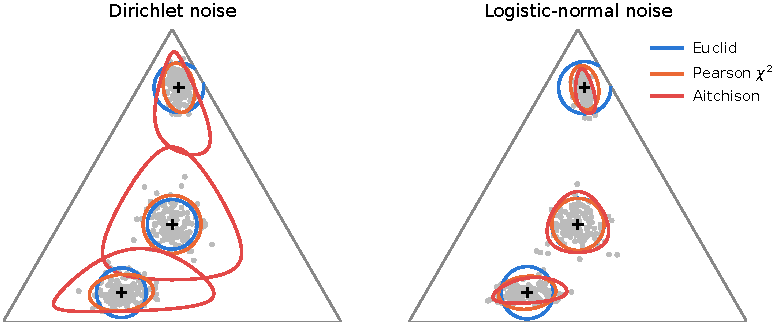
\includegraphics[width=\linewidth]{figs/fig_ternary.pdf}
\caption{Marginally calibrated (90\%) regions on the 3-part simplex for three predictions $\yh$ (+) under Dirichlet (left) and logistic-normal (right) noise, for three scores; grey: simulated targets. All regions have the same marginal coverage; their shapes, and hence conditional coverage, differ.}\label{fig:ternary}
\end{figure}

\subsection{Matching geometry to noise (oracle predictor)}\label{sec:e2}
\textbf{Design.} $X\sim N(0,I_5)$, $\mu(x)=\mathrm{softmax}(1.5(A x+B\sin Cx))$ with random $A,B,C$; $Y\mid x$ from (i) $\Dir(\kappa\mu)$, (ii) logistic-normal around $\mu$, (iii) additive Gaussian around $\mu$ truncated to the simplex (components of $\mu$ floored at $0.3/D$); (ii) and (iii) have noise matched to the Dirichlet in mean squared error. $D\in\{3,5,10\}$, $\kappa\in\{30,100,300,1000\}$; $\hat y=\mu(x)$; $n=1000$; five problem instances (random $A,B,C$) $\times$ 100 calibration draws, 40{,}000 test points, 150 centres for P3. $G$ is the larger of the worst gaps over confidence deciles and deciles of $\log\min_i\yh_i$.

\begin{table}[t]
\caption{Oracle predictor, split conformal, $n{=}1000$, $\alpha{=}0.1$. $G$: worst-slice gap (floor $\approx0.012$--$0.02$ from 40k test points); $\Delta\log$mass: mean log $M_1$ minus that of the best score in the same setting (nats). Mean $\pm$ 95\% $t$-interval over 5 problem instances; bold: smallest $G$ (within $0.0025$) / within $0.05$ nats of the best. Full grid: App.\ \cref{tab:e2fullG,tab:e2fulldlm}.}\label{tab:e2}
\centering\scriptsize
\resizebox{\columnwidth}{!}{\begin{tabular}{lcccc}\toprule
 & \multicolumn{2}{c}{$D{=}5,\kappa{=}100$} & \multicolumn{2}{c}{$D{=}10,\kappa{=}300$}\\
\cmidrule(lr){2-3}\cmidrule(lr){4-5}
score & $G$ & $\Delta\!\log$mass & $G$ & $\Delta\!\log$mass\\\midrule
\multicolumn{5}{l}{\emph{Dirichlet noise}}\\
Euclid & $0.090\,{\scriptstyle\pm0.011}$ & $1.25\,{\scriptstyle\pm0.57}$ & $0.086\,{\scriptstyle\pm0.005}$ & $3.35\,{\scriptstyle\pm1.02}$\\
TV & $0.102\,{\scriptstyle\pm0.015}$ & $1.14\,{\scriptstyle\pm0.55}$ & $0.123\,{\scriptstyle\pm0.023}$ & $2.78\,{\scriptstyle\pm0.88}$\\
Hellinger & $0.045\,{\scriptstyle\pm0.020}$ & $0.25\,{\scriptstyle\pm0.23}$ & $0.048\,{\scriptstyle\pm0.009}$ & $0.36\,{\scriptstyle\pm0.29}$\\
Pearson $\chi^2$ & $\mathbf{0.018}\,{\scriptstyle\pm0.004}$ & $\mathbf{0.00}\,{\scriptstyle\pm0.00}$ & $\mathbf{0.025}\,{\scriptstyle\pm0.004}$ & $\mathbf{0.03}\,{\scriptstyle\pm0.05}$\\
KL & $0.036\,{\scriptstyle\pm0.013}$ & $0.09\,{\scriptstyle\pm0.13}$ & $0.040\,{\scriptstyle\pm0.009}$ & $0.09\,{\scriptstyle\pm0.14}$\\
Aitchison & $0.410\,{\scriptstyle\pm0.118}$ & $5.57\,{\scriptstyle\pm2.49}$ & $0.419\,{\scriptstyle\pm0.141}$ & $15.10\,{\scriptstyle\pm1.82}$\\
\addlinespace[2pt]
\multicolumn{5}{l}{\emph{Logistic-normal noise}}\\
Euclid & $0.095\,{\scriptstyle\pm0.008}$ & $3.62\,{\scriptstyle\pm1.05}$ & $0.083\,{\scriptstyle\pm0.010}$ & $13.21\,{\scriptstyle\pm7.00}$\\
TV & $0.098\,{\scriptstyle\pm0.007}$ & $3.27\,{\scriptstyle\pm1.03}$ & $0.092\,{\scriptstyle\pm0.006}$ & $11.30\,{\scriptstyle\pm6.79}$\\
Hellinger & $0.092\,{\scriptstyle\pm0.012}$ & $1.68\,{\scriptstyle\pm0.65}$ & $0.086\,{\scriptstyle\pm0.005}$ & $6.99\,{\scriptstyle\pm5.97}$\\
Pearson $\chi^2$ & $0.088\,{\scriptstyle\pm0.015}$ & $1.45\,{\scriptstyle\pm0.44}$ & $0.083\,{\scriptstyle\pm0.006}$ & $6.60\,{\scriptstyle\pm5.73}$\\
KL & $0.091\,{\scriptstyle\pm0.013}$ & $1.58\,{\scriptstyle\pm0.57}$ & $0.085\,{\scriptstyle\pm0.006}$ & $6.83\,{\scriptstyle\pm5.89}$\\
Aitchison & $\mathbf{0.017}\,{\scriptstyle\pm0.003}$ & $\mathbf{0.00}\,{\scriptstyle\pm0.00}$ & $\mathbf{0.017}\,{\scriptstyle\pm0.002}$ & $\mathbf{0.00}\,{\scriptstyle\pm0.00}$\\
\addlinespace[2pt]
\multicolumn{5}{l}{\emph{Additive noise}}\\
Euclid & $0.035\,{\scriptstyle\pm0.010}$ & $\mathbf{0.00}\,{\scriptstyle\pm0.00}$ & $0.032\,{\scriptstyle\pm0.005}$ & $\mathbf{0.00}\,{\scriptstyle\pm0.00}$\\
TV & $\mathbf{0.032}\,{\scriptstyle\pm0.007}$ & $0.09\,{\scriptstyle\pm0.01}$ & $\mathbf{0.027}\,{\scriptstyle\pm0.002}$ & $0.34\,{\scriptstyle\pm0.01}$\\
Hellinger & $0.082\,{\scriptstyle\pm0.006}$ & $0.60\,{\scriptstyle\pm0.09}$ & $0.130\,{\scriptstyle\pm0.027}$ & $1.67\,{\scriptstyle\pm0.19}$\\
Pearson $\chi^2$ & $0.076\,{\scriptstyle\pm0.007}$ & $0.34\,{\scriptstyle\pm0.06}$ & $0.138\,{\scriptstyle\pm0.028}$ & $0.98\,{\scriptstyle\pm0.15}$\\
KL & $0.078\,{\scriptstyle\pm0.008}$ & $0.45\,{\scriptstyle\pm0.07}$ & $0.135\,{\scriptstyle\pm0.025}$ & $1.25\,{\scriptstyle\pm0.15}$\\
Aitchison & $0.123\,{\scriptstyle\pm0.013}$ & $2.18\,{\scriptstyle\pm0.32}$ & $0.152\,{\scriptstyle\pm0.042}$ & $6.13\,{\scriptstyle\pm0.56}$\\
\addlinespace[2pt]
\bottomrule\end{tabular}
}
\end{table}

\textbf{Results.} Marginal coverage is valid throughout (mean over the $1.05\times10^5$ split-conformal rows $0.9009$; SD across draws $0.0093$ vs.\ the Beta value $0.0095$). The matched geometry gives the smallest region in 35/35 cells and in each of the 175 problem instances (Dirichlet $\to$ Fisher-type, mostly $\chi^2$ and KL; logistic-normal $\to$ Aitchison; additive $\to$ Euclid) and the smallest $G$ within that family in 33/35 (\cref{tab:e2}; Euclid and TV count as one family; the two exceptions are additive noise at $D{=}5,\kappa{=}30$ and $D{=}10,\kappa{=}100$, where truncation matters). The price of the wrong geometry is large: under Dirichlet noise the Aitchison score is $5.6\pm2.5$ nats ($D{=}5$) and $15.1\pm1.8$ nats ($D{=}10$) worse in log-mass and has $G\approx0.4$; Euclid is $1.3$--$3.4$ nats worse with $G\approx0.09$. Under logistic-normal noise, the Fisher scores, TV and Euclid are $1.5$--$13$ nats worse in Table~\ref{tab:e2} ($0.4$--$21$ over the whole grid). The class of the winner is the same under the Jeffreys measure $a=\tfrac12$ in 33/35 cells; the exceptions are again low-$\kappa$ additive cells. Among Fisher-type scores the identity of the best one depends on the measure ($\chi^2$ for $a=1$, KL/Hellinger for $a=\tfrac12$), with differences up to $1.3$ nats (Hellinger, $a=1$) and $0.3$ nats ($a=\tfrac12$).

\textbf{Ellipsoidal baseline.} A standard multi-output choice is a Mahalanobis score with a global residual covariance \citep{johnstone2022,xu2024}; we fit it in ilr coordinates on 2000 extra points (App.\ \cref{tab:e2d}, $D\in\{5,10\}$, $\kappa\in\{100,300\}$). It reproduces the Aitchison score to within $0.025$ in $G$ and $0.13$ nats in all 12 cells (e.g.\ Dirichlet $D{=}10$, $\kappa{=}300$: $G=0.405$ vs $0.419$, $\Delta\log M_1=15.06$ vs $15.10$): the problem is the dependence of the noise scale on $\mu$, not anisotropy, which a global covariance cannot remove.

\subsection{Theory check}\label{sec:theorycheck}
For Dirichlet noise we compare the conditional coverage per confidence decile at the exact marginal radius to the prediction from the Gaussian limit of \cref{prop:pivot} (400{,}000 draws per cell). For $\kappa\ge300$ and $D\le5$ the largest discrepancy over deciles is $\le0.010$ for all scores (App.\ \cref{tab:e2b}); for $D=10$, where $\kappa\mu_{\min}$ is small, it is up to $0.05$ for Aitchison and $0.075$ for Hellinger at $\kappa=30$ and $\le0.025$ at $\kappa\ge1000$. \cref{fig:theory} shows the predicted curves and exact simulations: coverage rises from $0.82$ to $1.0$ with confidence for Euclid/TV, falls from $1.0$ to $0.6$ for Aitchison, and is flat for $\chi^2$.

\begin{figure}[t]
\centering
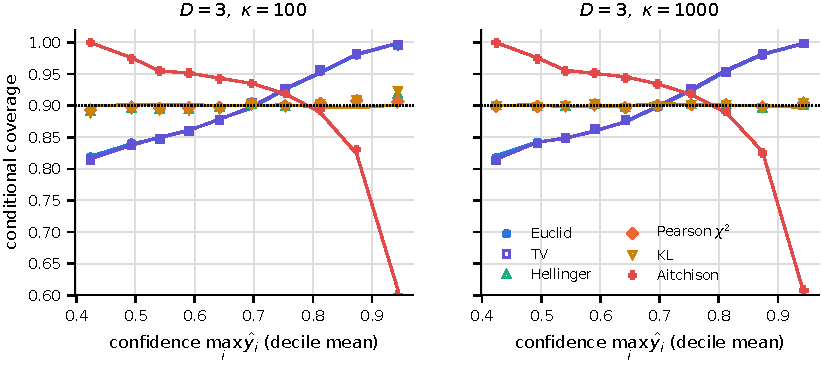
\includegraphics[width=\linewidth]{figs/fig_theory.pdf}
\caption{Conditional coverage by confidence decile, Dirichlet noise, $D=3$: exact simulation (markers) vs.\ Gaussian-limit prediction (lines) of \cref{prop:pivot}.}\label{fig:theory}
\end{figure}

\subsection{Zeros and predictor misfit}\label{sec:misfit}
\textbf{Count noise with zeros.} Dirichlet--multinomial targets ($Y=\text{counts}/N_{\rm ann}$, $p\sim\Dir(\kappa\mu)$) with $N_{\rm ann}\in\{10,50\}$, $\kappa\in\{30,300\}$, $D\in\{5,10\}$ have 17--60\% exact zeros. With the oracle $\yh=\mu$, $\chi^2$ has the smallest $G$ ($0.022$--$0.038$) and the smallest region in all 8 cells; KL is next ($0.3$--$1.4$ nats larger), Aitchison with $\delta\in\{10^{-3},10^{-2}\}$ is $1.6$--$7.3$ nats larger with $G=0.06$--$0.24$ (App.\ \cref{tab:e2c}). Zeros alone do not remove the Fisher advantage when $\yh$ is the true conditional centre.

\textbf{Predictor misfit.} We now let the predictor be $\yh(x)=\mathrm{softmax}\big((\log\mu(x)+s_{\rm err}\,h(x))/T\big)$ with a fixed smooth unit-variance random $h$ and $T<1$ over-confident (Dirichlet--multinomial targets, $N_{\rm ann}=50$, $\kappa=100$, $D=10$; slices use $\yh$). \cref{tab:misfit} shows that the smallest region remains the $\chi^2$ one in every setting, whereas its conditional gap grows from $0.03$ to $0.28$--$0.31$ for the over-confident predictors and the best $G$ moves to Aitchison ($\delta=10^{-2}$, $0.06$--$0.08$). So the oracle ranking does not transfer to misfit predictors, and size ranks the geometries differently from conditional validity.

\begin{table}[t]
\caption{Predictor misfit (E3b), $D=10$. $s_{\rm err}$: logit error scale, $T$: temperature of the predictor, $\mathrm{KL}_{\rm pred}$: mean $\mathrm{KL}(\mu\|\yh)$. Per setting, first line $G$ (max over confidence and min-component deciles; floor $\approx0.02$), second line $\Delta\log M_1$ (nats, relative to the best score); mean over 5 problems $\times$ 100 draws; bold: best.}\label{tab:misfit}
\centering\scriptsize\resizebox{\columnwidth}{!}{\begin{tabular}{rrrcccccc}\toprule
$s_{\rm err}$ & $T$ & $\mathrm{KL}_{\rm pred}$ & Euclid & TV & Hellinger & Pearson $\chi^2$ & KL & Ait. $10^{-2}$\\\midrule
0 & 1 & 0.00 & $0.082$ & $0.122$ & $0.081$ & $\mathbf{0.029}$ & $0.071$ & $0.072$\\
 & & & $2.64$ & $2.37$ & $2.76$ & $\mathbf{0.00}$ & $0.97$ & $3.83$\\[-1pt]
1 & 0.5 & 0.79 & $0.149$ & $0.119$ & $0.102$ & $0.278$ & $0.169$ & $\mathbf{0.062}$\\
 & & & $4.13$ & $3.55$ & $2.78$ & $\mathbf{0.00}$ & $1.13$ & $3.35$\\[-1pt]
1 & 1 & 0.20 & $0.090$ & $0.081$ & $0.074$ & $0.133$ & $0.077$ & $\mathbf{0.067}$\\
 & & & $2.97$ & $2.40$ & $2.08$ & $\mathbf{0.00}$ & $0.90$ & $2.42$\\[-1pt]
2 & 0.5 & 2.00 & $0.142$ & $0.119$ & $0.103$ & $0.307$ & $0.193$ & $\mathbf{0.079}$\\
 & & & $2.71$ & $2.38$ & $2.21$ & $\mathbf{0.00}$ & $1.04$ & $2.60$\\[-1pt]
\bottomrule\end{tabular}
}
\end{table}

\subsection{Learned predictors, heteroscedastic noise, adaptive methods, selection}\label{sec:e3}
\textbf{Adaptive methods.} With an MLP predictor (soft cross-entropy; $n_{\rm train}\in\{300,3000\}$; mean KL to the truth $0.012$ / $0.0024$), $D{=}5$, $\kappa{=}100$ and noise SD multiplied by $s(x)=e^{\tanh(v^\top x)}\in[e^{-1},e]$, we compare plain split, Studentised scores ($s/\hat\sigma(x)$, $\hat\sigma$ from a gradient-boosted model fit on a disjoint set), Mondrian by deciles of $\hat\sigma(x)$, and Mondrian by confidence (\cref{tab:e3}, $n_{\rm train}=3000$; 5 problems $\times$ 100 draws). Under heteroscedasticity the slice gap over $s(x)$ deciles is $0.29$ for $\chi^2$ split and $0.27$ for Mondrian-by-confidence, vs.\ $0.06$ (Studentised) and $0.05$ (Mondrian by $\hat\sigma$), while the region log-mass \emph{decreases} by $1.2\pm0.3$ nats; Mondrian by confidence does not help because the heteroscedasticity is not a function of $\yh$. Under homoscedastic noise, Studentising costs $0.01\pm0.02$ nats for $\chi^2$. Studentising does not repair a wrong geometry (Studentised Aitchison under Dirichlet noise stays $2.5\pm1.9$ nats (heteroscedastic) and $4.0\pm1.4$ nats (homoscedastic) larger than split $\chi^2$).

\begin{table}[t]
\caption{Learned MLP predictor ($n_{\rm train}=3000$), Dirichlet noise, $D{=}5$, $\kappa{=}100$; $G_{s(x)}$: worst gap over deciles of the true noise scale, $G_{\rm conf}$: over confidence deciles; $\Delta$ log mass relative to plain split of the same score (paired over problems, $\pm$ 95\% $t$ interval). Other families: App.\ \cref{tab:e3full}.}\label{tab:e3}
\centering\scriptsize
\resizebox{\columnwidth}{!}{\begin{tabular}{llcccc}\toprule
score & method & cov. & $G_{s(x)}$ & $G_{\rm conf}$ & $\Delta$ log mass\\\midrule
Pearson $\chi^2$ & split & 0.899 & 0.286 & 0.025 & $0.00\,{\scriptstyle\pm0.00}$\\
Pearson $\chi^2$ & Studentised & 0.900 & 0.063 & 0.033 & $-1.23\,{\scriptstyle\pm0.30}$\\
Pearson $\chi^2$ & Mondrian (pred. scale) & 0.904 & 0.047 & 0.030 & $-1.17\,{\scriptstyle\pm0.33}$\\
Pearson $\chi^2$ & Mondrian (confidence) & 0.904 & 0.265 & 0.056 & $0.07\,{\scriptstyle\pm0.05}$\\
Aitchison & split & 0.901 & 0.270 & 0.191 & $0.00\,{\scriptstyle\pm0.00}$\\
Aitchison & Studentised & 0.902 & 0.064 & 0.054 & $-2.64\,{\scriptstyle\pm0.37}$\\
Aitchison & Mondrian (pred. scale) & 0.906 & 0.057 & 0.040 & $-2.70\,{\scriptstyle\pm0.51}$\\
Aitchison & Mondrian (confidence) & 0.905 & 0.251 & 0.057 & $-0.36\,{\scriptstyle\pm0.14}$\\
\bottomrule\end{tabular}
}
\end{table}

\textbf{Score selection.} A user may choose among geometries from data. We take 8 candidates (Box--Cox/power distances $\|y^\lambda-\yh^\lambda\|/\lambda$ with $\lambda\in\{1,\tfrac34,\tfrac12,\tfrac14\}$, $\chi^2$, KL, TV, Aitchison) and compare (i) choosing by estimated log-mass on the \emph{same} data used to calibrate, (ii) choosing on one half and calibrating on the other, (iii) fixed scores, (iv) an oracle (\cref{tab:e4}, $n=1000$, 5 problems $\times$ 300 draws, test pool $4\times10^5$). Naive selection is within $0.01$ nats of the oracle in size but loses $0.13\pm0.02$ (Dirichlet $D{=}5$) and $0.16\pm0.02$ points of coverage relative to it (paired); honest splitting keeps validity but widens the SD of coverage by $\approx40\%$ ($0.94\to1.3$ points) at $\le0.02$ nats cost. The effect is small relative to calibration noise ($0.9$ pts), so the main risk of choosing the geometry on the calibration data is modest for small candidate sets; we conjecture it grows with the number of near-tied candidates (not tested).

\subsection{Real human label distributions}\label{sec:real}
\textbf{Data and predictors.} CIFAR-10H \citep{peterson2019}: human label distributions (47--63 annotations) for the 10{,}000 CIFAR-10 test images \citep{krizhevsky2009}; $\yh=\mathrm{softmax}(z/T)$ for the pretrained ResNet-56 \citep{chenyaofo} (94.25\% accurate on the CIFAR-10 labels), $T$ fitted by CE to the human distributions on 1000 held-out images \citep{guo2017}; the remaining 9000 images are randomly split 2000 calibration / 7000 test, 100 repetitions. 80.6\% of the target entries are exactly zero and 44\% of targets are vertices. ChaosNLI \citep{nie2020}: 3113 SNLI/MNLI items with 100 annotations each (7.9\% zero entries) and softmax outputs of RoBERTa-large-MNLI (68\% agreement with the human majority) and a distilled model.
\textbf{Protocol application.} Slices: confidence deciles ($G_{\rm conf}$) and predicted class ($G_{\rm class}$). Per-image coverage is averaged over repetitions and bootstrapped over images; null gap $G_{\rm null}\approx0.021$ for one split.

\begin{table}[t]
\caption{Real human-label distributions, split conformal unless noted, $\alpha=0.1$. $G_{\rm conf},G_{\rm class}$: worst gap over confidence deciles / predicted classes, pooled over 100 random splits (null floor for one split: $0.021/0.021$ CIFAR-10H, $0.045/0.018$ ChaosNLI); log mass: mean $\log M_1$. Bootstrap intervals and other predictors: App.\ \cref{tab:cifarfull,tab:cifarother,tab:nlifull,tab:nliraw,tab:nlidistil,tab:alpha}.}\label{tab:real}
\centering\scriptsize
\resizebox{\columnwidth}{!}{\begin{tabular}{lcccccc}\toprule
 & \multicolumn{3}{c}{CIFAR-10H (ResNet-56, $D{=}10$)} & \multicolumn{3}{c}{ChaosNLI (roberta-large, $D{=}3$)}\\
\cmidrule(lr){2-4}\cmidrule(lr){5-7}
score & $G_{\rm conf}$ & $G_{\rm class}$ & log mass & $G_{\rm conf}$ & $G_{\rm class}$ & log mass\\\midrule
Euclid & 0.578 & 0.092 & -8.04 & 0.059 & 0.051 & -0.58\\
TV & 0.589 & 0.093 & -8.66 & 0.062 & 0.054 & -0.58\\
Hellinger & 0.606 & 0.094 & -7.13 & 0.048 & 0.036 & -0.53\\
Pearson $\chi^2$ & 0.217 & 0.129 & -13.15 & 0.081 & 0.053 & -0.70\\
KL & 0.457 & 0.093 & -10.36 & 0.065 & 0.050 & -0.64\\
Aitchison $\delta{=}10^{-4}$ & 0.321 & 0.130 & -0.12 & 0.042 & 0.046 & -0.00\\
Aitchison $\delta{=}10^{-2}$ & 0.472 & 0.097 & -5.79 & 0.057 & 0.041 & -0.31\\
Mahalanobis-ilr $\delta{=}10^{-2}$ & 0.461 & 0.074 & -6.21 & 0.035 & 0.058 & -0.37\\
Pearson $\chi^2$ (Mondrian conf.) & 0.009 & 0.153 & -14.55 & 0.013 & 0.042 & -0.65\\
Pearson $\chi^2$ (Mondrian class) & 0.228 & 0.005 & -13.08 & 0.069 & 0.003 & -0.70\\
\bottomrule\end{tabular}
}
\end{table}

\begin{figure}[t]
\centering
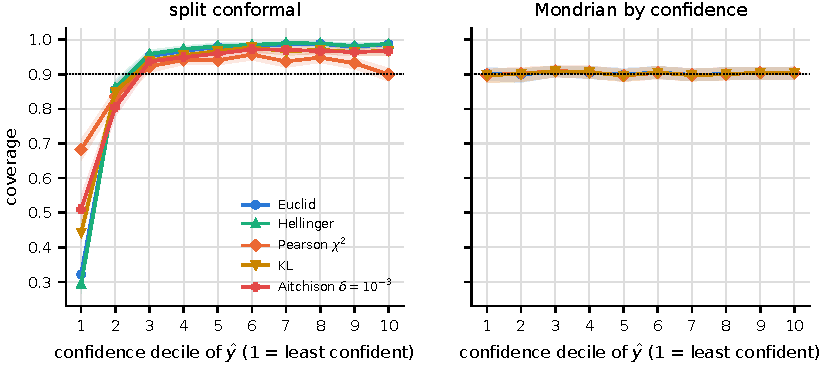
\includegraphics[width=\linewidth]{figs/fig_cifar.pdf}
\caption{CIFAR-10H, ResNet-56: coverage per confidence decile of $\yh$ for split conformal (left) and Mondrian by confidence (right); bands: 95\% bootstrap over images.}\label{fig:cifar}
\end{figure}

\textbf{CIFAR-10H.} All methods are marginally valid (coverage $0.899$--$0.903$, \cref{tab:real}), yet \cref{fig:cifar} shows that every split-conformal score under-covers the least confident decile (coverage $0.29$ Hellinger, $0.32$ Euclid, $0.44$ KL, $0.51$ Aitchison with $\delta=10^{-3}$, $0.68$ $\chi^2$) and over-covers confident images (up to $0.99$). $G_{\rm conf}$ is $0.22$--$0.61$ against a null floor of $0.021$, and it remains $\ge0.13$ for every predictor we tried (raw softmax, ResNet-20, VGG-11; App.\ \cref{tab:cifarfull}). Pearson $\chi^2$---the winner on synthetic Dirichlet data---is the least bad ($G_{\rm conf}=0.22$) and gives the smallest region ($\log M_1=-13.2$), but its coverage drifts \emph{down} again in the most confident decile ($0.90$), so Dirichlet-matched geometry does not transfer: 80\% of target entries are exact zeros, and 44\% of targets are vertices (where all Fisher-type scores coincide with LAC, \cref{prop:lac}).
Conditioning removes only the conditioned variable's gap: Mondrian by confidence reaches $G_{\rm conf}=0.009$ (below the null floor) but \emph{raises} $G_{\rm class}$ (Euclid $0.09\to0.13$, KL $0.09\to0.15$, $\chi^2$ $0.13\to0.15$) and gives much smaller regions on average (log-mass $-14.5$ to $-16.0$ vs.\ $-8.0$ to $-13.2$ unconditioned); Mondrian by predicted class reaches $G_{\rm class}=0.005$ and leaves $G_{\rm conf}$ at $0.2$--$0.5$.
The Aitchison score is \emph{not a single method}: with $\delta=10^{-4},10^{-3},10^{-2},10^{-1}$, $G_{\rm conf}=0.32,0.39,0.47,0.54$ and $\log M_1=-0.12,-1.9,-5.8,-6.6$; a region of log-mass $-0.12$ is essentially the whole simplex. A comparison of Aitchison against other geometries on zero-rich data is therefore a comparison with the choice of $\delta$. A global-covariance ellipsoid in ilr coordinates (fitted on the 1000 held-out images, $\delta=10^{-2}$) behaves like the Aitchison score ($G_{\rm conf}=0.46$ vs.\ $0.47$). The ranking is stable across $\alpha\in\{0.05,0.1,0.2\}$ ($\chi^2$ lowest $G_{\rm conf}$: $0.064,0.217,0.513$), but gaps grow with $\alpha$ (App.\ \cref{tab:alpha}).

\textbf{ChaosNLI} (\cref{tab:real}, right; RoBERTa-large, $T$ fitted on 500 items). With 3 components and 7.9\% zeros the picture differs: for all scores except $\chi^2$ the confidence gap ($0.035$--$0.065$) is close to the null floor of this test-set size ($0.045$); $\chi^2$ is worst ($0.081$, lowest-decile coverage $0.82$) \emph{while} giving the smallest region ($\log M_1=-0.70$ vs.\ $-0.53$ for Hellinger): size alone would pick the geometry with the worst conditional coverage, the situation P3 warns about. With the raw over-confident softmax ($T=1$) the gaps grow to $0.08$--$0.09$ (Euclid, TV, Hellinger, Mahalanobis), $0.15$ (KL), $0.22$ (Aitchison, $\delta=10^{-3}$) and $0.29$ ($\chi^2$, lowest-decile coverage $0.61$) with $\chi^2$ again the smallest region ($-1.03$), the pattern of the synthetic misfit experiment (\cref{sec:misfit}); the distilled model gives a similar picture at $T$ fitted ($\chi^2$ $0.10$, Mahalanobis with $\delta=10^{-3}$ $0.14$, the others $\le0.06$; App.\ \cref{tab:nlifull,tab:nliraw,tab:nlidistil}). The pattern is dataset-specific: on CIFAR-10H the raw softmax leaves $\chi^2$ best ($0.205$ vs.\ $0.23$--$0.46$ for the others). Regions are large in absolute terms because human label distributions on this subset are dispersed (geometric-mean mass $e^{-0.53}=0.59$ of the simplex for Hellinger and $e^{-0.70}=0.50$ for $\chi^2$ at fitted $T$).


\subsection{Covariate shift}\label{sec:shift}
We tilt the calibration set towards easy images: calibration images (1500 of a 4500 pool) are drawn with probability $\propto e^{\gamma u}$, $u$ the confidence rank; the test set is the uniform remaining half (200 repetitions; $\gamma$ up to 4, effective sample size 500). Split conformal coverage decays from $0.899$ to $0.870$ ($\chi^2$) and $0.760$ (Euclid) as $\gamma$ grows; weighted conformal \citep{tibshirani2019} with weights estimated by logistic regression on confidence features restores marginal coverage ($0.899$--$0.906$) but not conditional coverage: on the low-confidence half $\chi^2$ coverage stays at $0.87$ vs.\ $0.829$ unweighted at $\gamma=4$. Mondrian by confidence is nearly unaffected ($0.901$--$0.913$ in both halves) \emph{because the shift is a function of confidence by construction}; shifts in unmodelled features would not be absorbed (\cref{fig:shift}, App.\ \cref{tab:e5b}).

\begin{figure}[t]
\centering
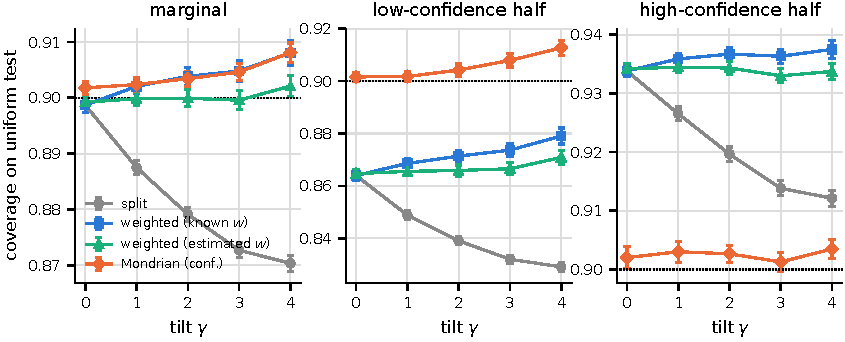
\includegraphics[width=\linewidth]{figs/fig_shift.pdf}
\caption{CIFAR-10H, Pearson $\chi^2$ score, covariate shift of strength $\gamma$ (mean $\pm$ 95\% CI over 200 splits).}\label{fig:shift}
\end{figure}

\section{Discussion and Limitations}
\textbf{What the evidence supports.} (1)~Coverage per se does not discriminate geometries and one-split evaluations are dominated by calibration noise. (2)~Geometry matters when noise is not degenerate: the Fisher-type scores are the right default for count/Dirichlet-like noise, Aitchison for multiplicative noise, Euclid for additive noise, and a wrong choice is paid in both size and conditional coverage. (3)~On CIFAR-10H (many exact zeros, mixtures of vertices and ambiguous items) and on over-confident NLI predictions, conditional coverage is poor for \emph{every} split-conformal score, and conditioning on the right variable (Mondrian) fixes only that variable; with a temperature-fitted NLI predictor all gaps are near the noise floor.

\textbf{When is which geometry preferable?} Summarising the evidence by condition (each row is supported by the cited experiment only): count-like (Dirichlet or Dirichlet--multinomial) noise around a well-calibrated predictor $\Rightarrow$ Pearson $\chi^2$ or KL (\cref{sec:e2,sec:misfit}); multiplicative log-ratio noise without exact zeros $\Rightarrow$ Aitchison (\cref{sec:e2}); additive noise far from the boundary $\Rightarrow$ Euclid or TV (\cref{sec:e2}); noise scale varying with unmodelled features $\Rightarrow$ Studentise or Mondrian by predicted scale on top of the geometry, not instead of it (\cref{sec:e3}); over-confident or misspecified predictor, or real label distributions $\Rightarrow$ no geometry was uniformly best, choose with held-out conditional diagnostics (\cref{sec:misfit,sec:real}). A mechanism consistent with the misfit result is that $\chi^2$ divides by $\yh_i$: confident-but-wrong predictions with tiny $\yh_i$ produce very large scores that dominate the quantile, whereas log-ratio distances are less sensitive to the scale of small components for a moderate $\delta$; we did not test this mechanism separately.

\textbf{Practical recommendations.} (i)~Report $V$'s spread, not a single-split coverage; (ii)~always report conditional gaps with their null floor, for slices that matter for the application, and read size only next to them; (iii)~preferably choose the geometry on data that is not used for calibration (App.~\ref{app:details}); (iv)~if a conditional requirement is known, condition on it (Mondrian) or Studentise, but expect other slices to move; (v)~treat zero-replacement constants as hyper-parameters and show the sensitivity; (vi)~re-evaluate with the deployed predictor, since oracle rankings need not transfer.

\textbf{Where not to extrapolate.} Our synthetic worlds use known noise families and $\alpha=0.1$, $D\le10$, $n=1000$; the asymptotics need $\kappa\mu_{\min}\gg1$ and fail for sparse compositions. Aitchison results depend on $\delta$ and on zero handling (\cref{sec:real}); we did not evaluate multiplicative replacement or Bayesian zero imputation. Size is measured under two reference measures and differs for the near-tied Fisher scores; a different measure may reorder close competitors, though never the geometry class in our grid except for two additive cells. The real-data results rely on two datasets with $D=10$ and $D=3$, off-the-shelf predictors, and exchangeability within a finite image pool; the bootstrap intervals for $G$ are unreliable below $\approx0.03$ (max statistic). We did not evaluate full conformal, jackknife+/CV+, learned (non-ball) scores, label-set methods for hard labels (APS/RAPS), or non-exchangeable data beyond the tilted shift. Selection of the geometry on calibration data inflates miscoverage by about $0.15$ points in our setting; we did not study larger candidate sets.

\section*{Impact Statement}
This paper presents work whose goal is to advance the field of Machine Learning. There are many potential societal consequences of our work, none which we feel must be specifically highlighted here.

\bibliography{refs}
\bibliographystyle{icml2026}

\newpage
\appendix
\onecolumn
\section{Proofs}\label{app:proofs}
\paragraph{Proof of \cref{prop:beta}.}
Let $U_i=F(S_i)$; for continuous $F$ the $U_i$ ($i\le n+1$) are exchangeable uniforms (iid in the standard split setting), $F(\hat q)=U_{(k)}$ is the $k$th order statistic of $n$ uniforms, distributed $\mathrm{Beta}(k,n+1-k)$ \citep{vovk2012}. With $l=n+1-k=\lfloor(n+1)\alpha\rfloor$ this is $\mathrm{Beta}(n+1-l,l)$, with mean $k/(n+1)\in[1-\alpha,1-\alpha+\tfrac1{n+1})$ and variance $k(n+1-k)/((n+1)^2(n+2))\approx\alpha(1-\alpha)/(n+2)$. Given $V$, the number of covered test points is $\mathrm{Bin}(m,V)$, so $\mathrm{Var}(\hat c)=\E[V(1-V)]/m+\mathrm{Var}(V)$ and $\E[V(1-V)]=\mu_V(1-\mu_V)-\mathrm{Var}(V)$.
\emph{Atoms.} Write $S_i=F^{-1}(U_i)$ with $U_i$ uniform. Then $F(F^{-1}(u))\ge u$, so the coverage $V=F(\hat q)=F(F^{-1}(U_{(k)}))\ge U_{(k)}$ pointwise: $V$ is stochastically larger than the Beta law, and has no upper bound near $1-\alpha+1/(n+1)$ (e.g.\ if every score equals one atom, $V=1$). \emph{Randomisation.} Draw independent $\xi_i\sim U(0,1)$ and order pairs $(S_i,\xi_i)$ lexicographically; the pairs are a.s.\ distinct and exchangeable, a test point is covered iff $(S_{n+1},\xi_{n+1})\le_{\rm lex}(\hat q,\hat\xi)$, and the argument for the continuous case applies to the rank of the test pair. $\square$

\paragraph{Proof of \cref{prop:pivot}.}
(a) $Y=G/\sum_jG_j$ with independent $G_i\sim\mathrm{Gamma}(\kappa\mu_i,1)$. By the CLT for gamma variables $\sqrt\kappa^{-1}(G_i-\kappa\mu_i)\Rightarrow Z_i\sim N(0,\mu_i)$ independent. With $S=\sum_jG_j$, $S/\kappa\to1$ and $\sqrt\kappa(Y_i-\mu_i)=\kappa^{-1/2}(G_i-\mu_iS)/(S/\kappa)\Rightarrow Z_i-\mu_i\sum_jZ_j$, a Gaussian with covariance $\mathrm{diag}(\mu)-2\mu\mu^\top+\mu\mu^\top=\Sigma(\mu)$. Put $W_i=Z_i/\sqrt{\mu_i}\sim N(0,1)$. Then $\kappa\sum_i(Y_i-\mu_i)^2/\mu_i\Rightarrow\sum_i(W_i-\sqrt{\mu_i}\,\sqrt\mu^\top W)^2=\|(I-\sqrt\mu\sqrt\mu^\top)W\|^2\sim\chi^2_{D-1}$ ($I-\sqrt\mu\sqrt\mu^\top$ is an orthogonal projector of rank $D-1$). Second-order expansions: $\|\sqrt y-\sqrt\mu\|^2=\sum_i(y_i-\mu_i)^2/(4\mu_i)+o(\|y-\mu\|^2)$ and $\mathrm{KL}(y\|\mu)=\tfrac12\sum_i(y_i-\mu_i)^2/\mu_i+o(\|y-\mu\|^2)$, which give the $\tfrac14\chi^2_{D-1}$ and $\tfrac12\chi^2_{D-1}$ limits (continuous mapping). Euclid: $\kappa\|Y-\mu\|^2\Rightarrow\|\Sigma^{1/2}Z\|^2=\sum_i\lambda_i(\Sigma)Z_i^2$, with mean $\mathrm{tr}\,\Sigma=1-\|\mu\|_2^2$. Aitchison: $\mathrm{clr}(y)-\mathrm{clr}(\mu)=P(\log y-\log\mu)=P\,\mathrm{diag}(1/\mu)(y-\mu)+o$, and the limiting covariance of $P\,\mathrm{diag}(1/\mu)\epsilon$ is $P\,\mathrm{diag}(1/\mu)\Sigma\,\mathrm{diag}(1/\mu)P=P(\mathrm{diag}(1/\mu)-\mathbf 1\mathbf 1^\top)P=P\,\mathrm{diag}(1/\mu)P$; its largest eigenvalue is $\ge(1-1/D)/\mu_{\min}$ (take the unit vector $v\propto Pe_j$ for the smallest component $j$). If $\mu$ ranges in a compact subset of the interior the convergences are uniform in $\mu$ (Berry--Esseen for the gamma sums, Lipschitz maps), so the (1$-\alpha$)-quantile $r_\kappa$ of $s$ under the mixture satisfies $\kappa r_\kappa^2\to c_s\chi^2_{D-1,1-\alpha}$ for the Fisher-type scores, and the conditional coverage $\Pr(s\le r_\kappa\mid\mu)\to1-\alpha$ uniformly. We have not proved rates; the non-asymptotic accuracy is evaluated numerically (\cref{sec:theorycheck}). (b),(c): $\|\mathrm{clr}(Y)-\mathrm{clr}(\mu)\|^2=\sigma^2\|P\varepsilon\|^2$ and $\|P\varepsilon\|^2\sim\chi^2_{D-1}$ for the rank-$(D{-}1)$ projector $P$; the distribution does not depend on $\mu$, so the marginal radius equals the conditional one for every $\mu$. $\square$

\paragraph{Proof of \cref{prop:lac}.} For $y=e_k$, $p=\yh_k$: $\sum_i(y_i-\yh_i)^2/\yh_i=(1-p)^2/p+\sum_{i\ne k}\yh_i=(1-p)^2/p+(1-p)=(1-p)/p$; $\|\sqrt y-\sqrt{\yh}\|^2=(1-\sqrt p)^2+(1-p)=2-2\sqrt p$; $\mathrm{TV}=\tfrac12[(1-p)+(1-p)]=1-p$; $\mathrm{KL}(e_k\|\yh)=-\log p$; each is strictly decreasing in $p$ so $\{k:s(e_k,\yh)\le\hat q\}=\{k:\yh_k\ge\tau\}$ for a threshold $\tau$ determined by the calibration scores, which is the LAC set. $\square$

\section{Experimental details}\label{app:details}
\paragraph{Synthetic problems.} $X\sim N(0,I_5)$; logits $z=1.5\,(A^\top x+B^\top\sin(C x))$, $A,B\in\mathbb R^{5\times D}$, $C\in\mathbb R^{5\times5}$ with $N(0,1/5)$ entries (fixed by the problem seed); $\mu=\mathrm{softmax}(z)$ (additive family: $\mu\leftarrow0.7\mu+0.3/D$). Dirichlet: $Y\sim\Dir(\kappa\mu)$ (gamma sampler). Logistic-normal: $\mathrm{clr}(Y)=\mathrm{clr}(\mu)+\sigma P\varepsilon$. Additive: $Y=\mu+\sigma P\varepsilon$, rejected until $Y_i>10^{-6}$ (all rows resampled until valid; the code asserts that fewer than $10^{-3}$ rows need the fallback $Y=\mu$). $\sigma$ is chosen by bisection so that $\E\|Y-\mu\|^2$ equals the Dirichlet value $\E(1-\|\mu\|^2)/(\kappa+1)$; the additive family with $D=10,\kappa=30$ is omitted because the truncation made matching impossible (35 cells instead of 36). Heteroscedastic variants (E3) multiply the noise SD by $s(x)=\exp(\tanh(v^\top x))$ ($\kappa\to\kappa/s^2$ for Dirichlet, $\sigma\to s\sigma$ for logistic-normal).
\paragraph{E2 slices.} Deciles of $\max_i\yh_i$ and of $\log\min_i\yh_i$ defined on the test pool; $G=\max$ over both slicings; Mondrian-by-confidence results for the same grid are in the released CSV (\texttt{e2\_geometry.csv}) but not discussed in the text.
\paragraph{Reference-mass estimator.} $M_a(C)=\Pr_{\Dir(a\mathbf 1)}(Y\in C)$ is estimated with $N=7\times1500$ draws from the mixture $q=\tfrac17\big[\Dir(a\mathbf1)+\sum_{\kappa\in\{5,20,100,500,2500,12500\}}\Dir(\kappa\yh+\mathbf 1)\big]$ and weights $\Dir(a\mathbf1)/q\le7$ (balance heuristic), one sample set per centre shared by all scores and all radii. Check against exact ball areas in the 3-simplex (50 seeds, \texttt{check\_mass\_estimator.py}): relative bias $\le0.2\%$, relative SD $1.5$--$1.8\%$ per centre. ESS over all centres and settings was $\ge1700$. Log-masses are averaged over 150 (synthetic) or 300 (real) centres; masses are floored at $10^{-300}$ (never active).
\paragraph{E1.} Dirichlet $D=3$, $\kappa=100$, oracle $\yh$; $R=5000$ draws per $n$; $V$ is measured on a pool of $2\times10^6$ test points. Lattice experiment: $Y=\text{counts}/N_{\rm ann}$ with counts $\sim$ Multinomial$(N_{\rm ann},p)$, $p\sim\Dir(20\cdot(0.5,0.3,0.2))$, constant predictor $(0.5,0.3,0.2)$, $n=1000$, 1000 draws, test pool $2\times10^5$. Mis-ranking: exact Beta/Binomial simulation, two predictors with nominal levels $0.90$ and $0.90+$gap, `indep': independent calibration sets, `paired': one shared calibration sample (order statistics $k_A<k_B$ of the same $n$ uniforms), $2\times10^5$ (indep) / $2\times10^4$ (paired) trials. A first run of E1 with a $4\times10^5$-point test pool (file \texttt{old\_e1a.csv}) rejected $\chi^2$ and Aitchison at $n=2000$ (mean $V$ shifts $+0.0006$ for $\chi^2$, $+0.0003$ for Aitchison); with the $2\times10^6$ pool $\chi^2$, KL and Aitchison rejected (shifts $-0.0004$, $-0.0003$, $+0.0006$). For $\chi^2$ and KL the sign and size of the shift change with the pool, consistent with pool sampling error (SE $5\times10^{-4}$ and $2\times10^{-4}$). The re-check \texttt{exp1b\_pool\_check.py} (pool $2\times10^7$, SE $7\times10^{-5}$, same calibration seeds) gives KS $p=0.61,0.68,0.32,0.39,0.08$ for Euclid, TV, Hellinger, $\chi^2$, KL and $p=0.005$ for Aitchison (mean $V=0.90024$ vs.\ $0.90005$, SD $0.00663$ vs.\ $0.00670$): we have no explanation for the Aitchison deviation; its size ($0.03$ SD of $V$) is negligible for the conclusions.
\paragraph{E3.} MLP: 2 hidden layers of 64 tanh units, Adam (lr $5\times10^{-3}$, weight decay $10^{-4}$), batch 256, 400 epochs, soft cross-entropy. Scale model $\hat\sigma(x)$: gradient boosting regression of $\log s$ on $[x,\mathrm{clr}(\yh)]$ (150 trees, depth 3, lr 0.05, subsample 0.8), fit on 2000 points disjoint from the MLP training set and the calibration set; Mondrian-by-scale bins are deciles of $\hat\sigma$ on the test pool. 5 problems $\times$ 100 calibration draws of $n=1000$, 40{,}000 test points.
\paragraph{E4.} Candidates: Box--Cox distances $\|y^\lambda-\yh^\lambda\|_2/\lambda$ for $\lambda\in\{1,0.75,0.25\}$ plus Hellinger ($\lambda=\tfrac12$), $\chi^2$, KL, TV, Aitchison. Selection criterion: mean $\log M_1$ over 150 fixed centres of the region at the candidate's calibration quantile. Naive: quantiles from all $n=1000$ points; honest: selection quantiles from the first 500, final quantile from the last 500; oracle: best candidate at its population quantile. $D\in\{5,10\}$ ($\kappa=100,300$), 5 problems $\times$ 300 draws, test pool $4\times10^5$.
\paragraph{Real data.} CIFAR-10H: counts normalised (47--63 annotations per image), CIFAR-10 test images from the Hugging Face mirror \texttt{uoft-cs/cifar10} (see \cref{app:repro}); 1000 images (fixed permutation, seed 0) fit the temperature $T$ (bounded scalar optimisation of CE against the soft labels); the other 9000 are re-split per repetition (seed $[5,r]$) into 2000 calibration / 7000 test. Fixed analysis slices: deciles of $\max\yh$ over the image pool, predicted class. ChaosNLI: SNLI (1514) + MNLI-m (1599) items; the human label order is $(e,n,c)$; 500 items fit $T$, 1000 calibration, remaining 1613 test. Aitchison: additive replacement $y\leftarrow(y+\delta\mathbf 1)/(1+D\delta)$ applied to both $y$ and $\yh$. Pooled per-image coverage (average over repetitions in which the image was a test image) is bootstrapped over images (200 resamples, percentile intervals); log-mass intervals bootstrap the 300 centres. Percentile bootstrap intervals for a max-type statistic such as $G$ are biased upward when the true value is below the noise floor (e.g.\ $G_{\rm conf}=0.009$ with interval $[0.011,0.030]$ for Mondrian by confidence): they are shown for reference only.
\paragraph{Shift.} Pool: 9000 images, split each repetition into calibration pool 4500 / test 4500; calibration points drawn without replacement with probabilities $\propto e^{\gamma u}$, $u\in[0,1]$ the confidence rank; known weights $w=1/\pi(x)\propto e^{-\gamma u}$; estimated weights: logistic regression (C=10) of calibration-vs-test on $[\log(1-\text{conf}),\log\text{entropy},u]$, odds clipped to $[10^{-3},10^3]$. This ignores the finite-population (without-replacement) correction.

\section{Additional results}
\begin{table}[h]
\caption{E1: calibration law. Mean/SD of coverage given calibration ($R=5000$ draws, $2\times10^6$ test points) vs.\ Beta; max KS statistic and min $p$ over the six scores.}\label{tab:e1a}
\centering\small\begin{tabular}{rcccccc}\toprule
$n$ & mean $V$ & Beta mean & SD $V$ & Beta SD & max KS & min $p$\\\midrule
20 & 0.9049 & 0.9048 & 0.0626 & 0.0626 & 0.016 & 0.177\\
50 & 0.9019 & 0.9020 & 0.0411 & 0.0412 & 0.017 & 0.113\\
100 & 0.9007 & 0.9010 & 0.0296 & 0.0296 & 0.019 & 0.055\\
500 & 0.9001 & 0.9002 & 0.0135 & 0.0134 & 0.019 & 0.057\\
2000 & 0.8999 & 0.9000 & 0.0067 & 0.0067 & 0.046 & 0.000\\
\bottomrule\end{tabular}

\end{table}
\begin{table}[h]
\caption{E1: lattice-valued compositions ($n=1000$): mean coverage and KS distance to the Beta law without and with randomised tie-breaking; \#atoms = distinct score values in the test pool. KS critical value at 5\%: $0.043$ for 1000 draws.}\label{tab:e1b}
\centering\small\begin{tabular}{rlrcccc}\toprule
$N_{\rm ann}$ & score & \#atoms & mean cov. & KS & mean cov. (rand.) & KS (rand.)\\\midrule
5 & Pearson $\chi^2$ & 18 & 0.9123 & 0.54 & 0.8990 & 0.057\\
5 & Euclid & 15 & 0.9580 & 1.00 & 0.8996 & 0.051\\
10 & Pearson $\chi^2$ & 54 & 0.9095 & 0.56 & 0.9010 & 0.054\\
10 & Euclid & 31 & 0.9079 & 0.49 & 0.9009 & 0.044\\
20 & Pearson $\chi^2$ & 175 & 0.9028 & 0.27 & 0.8997 & 0.024\\
20 & Euclid & 86 & 0.9101 & 0.47 & 0.8997 & 0.036\\
50 & Pearson $\chi^2$ & 710 & 0.8999 & 0.06 & 0.8993 & 0.053\\
50 & Euclid & 324 & 0.9019 & 0.20 & 0.9001 & 0.027\\
\bottomrule\end{tabular}

\end{table}
\begin{table}[h]
\caption{E1: probability that a method with nominal coverage $0.90+$gap is \emph{observed} to cover no more than a method with nominal $0.90$ on one split: ``independent calibration sets / shared calibration set''; $n$ calibration, $m$ test points.}\label{tab:e1c}
\centering\small\begin{tabular}{rrccc}\toprule
$n$ & $m$ & gap 0.01 & gap 0.02 & gap 0.05\\\midrule
100 & 500 & 0.42 / 0.34 & 0.33 / 0.19 & 0.11 / 0.02\\
100 & 2000 & 0.41 / 0.23 & 0.31 / 0.09 & 0.09 / 0.00\\
100 & 10000 & 0.40 / 0.13 & 0.31 / 0.03 & 0.08 / 0.00\\
500 & 500 & 0.36 / 0.32 & 0.23 / 0.16 & 0.02 / 0.00\\
500 & 2000 & 0.32 / 0.17 & 0.16 / 0.03 & 0.00 / 0.00\\
500 & 10000 & 0.30 / 0.04 & 0.14 / 0.00 & 0.00 / 0.00\\
2000 & 500 & 0.33 / 0.32 & 0.17 / 0.15 & 0.00 / 0.00\\
2000 & 2000 & 0.23 / 0.15 & 0.06 / 0.02 & 0.00 / 0.00\\
2000 & 10000 & 0.16 / 0.02 & 0.02 / 0.00 & 0.00 / 0.00\\
\bottomrule\end{tabular}

\end{table}
\begin{table}[h]
\caption{E2b: largest absolute difference (over confidence deciles) between the conditional coverage predicted from the Gaussian limit and the exact Dirichlet simulation, at the exact marginal radius.}\label{tab:e2b}
\centering\small\begin{tabular}{rrcccccc}\toprule
$D$ & $\kappa$ & Euclid & TV & Hellinger & Pearson $\chi^2$ & KL & Aitchison\\\midrule
3 & 30 & 0.008 & 0.007 & 0.044 & 0.006 & 0.039 & 0.012\\
3 & 100 & 0.007 & 0.006 & 0.017 & 0.011 & 0.022 & 0.009\\
3 & 300 & 0.005 & 0.005 & 0.006 & 0.006 & 0.010 & 0.005\\
3 & 1000 & 0.003 & 0.004 & 0.004 & 0.007 & 0.007 & 0.003\\
3 & 3000 & 0.002 & 0.003 & 0.004 & 0.005 & 0.005 & 0.002\\
5 & 30 & 0.009 & 0.007 & 0.036 & 0.010 & 0.028 & 0.013\\
5 & 100 & 0.007 & 0.003 & 0.016 & 0.007 & 0.016 & 0.010\\
5 & 300 & 0.003 & 0.004 & 0.009 & 0.003 & 0.010 & 0.003\\
5 & 1000 & 0.003 & 0.002 & 0.004 & 0.005 & 0.004 & 0.004\\
5 & 3000 & 0.004 & 0.005 & 0.003 & 0.003 & 0.003 & 0.003\\
10 & 30 & 0.009 & 0.006 & 0.075 & 0.020 & 0.053 & 0.051\\
10 & 100 & 0.004 & 0.004 & 0.053 & 0.023 & 0.039 & 0.031\\
10 & 300 & 0.003 & 0.002 & 0.041 & 0.017 & 0.034 & 0.008\\
10 & 1000 & 0.004 & 0.003 & 0.025 & 0.013 & 0.022 & 0.023\\
10 & 3000 & 0.004 & 0.005 & 0.013 & 0.007 & 0.013 & 0.013\\
\bottomrule\end{tabular}

\end{table}
\begin{table}[h]
\caption{E2: worst-slice gap $G$ for the full grid (oracle predictor, $n=1000$); mean over 5 problems $\times$ 100 draws; bold: smallest or within $0.0025$.}\label{tab:e2fullG}
\centering\scriptsize\begin{tabular}{llrcccccc}\toprule
noise & $D$ & $\kappa$ & Euclid & TV & Hellinger & Pearson $\chi^2$ & KL & Aitchison\\\midrule
Dirichlet & 3 & 30 & $0.095$ & $0.100$ & $0.050$ & $\mathbf{0.023}$ & $0.043$ & $0.404$\\
Dirichlet & 3 & 100 & $0.102$ & $0.104$ & $0.035$ & $\mathbf{0.019}$ & $0.034$ & $0.432$\\
Dirichlet & 3 & 300 & $0.101$ & $0.104$ & $0.023$ & $\mathbf{0.017}$ & $0.024$ & $0.427$\\
Dirichlet & 3 & 1000 & $0.102$ & $0.104$ & $\mathbf{0.018}$ & $\mathbf{0.017}$ & $\mathbf{0.018}$ & $0.415$\\
Dirichlet & 5 & 30 & $0.086$ & $0.104$ & $0.060$ & $\mathbf{0.022}$ & $0.049$ & $0.303$\\
Dirichlet & 5 & 100 & $0.090$ & $0.102$ & $0.045$ & $\mathbf{0.018}$ & $0.036$ & $0.410$\\
Dirichlet & 5 & 300 & $0.093$ & $0.104$ & $0.030$ & $\mathbf{0.016}$ & $0.028$ & $0.489$\\
Dirichlet & 5 & 1000 & $0.093$ & $0.103$ & $0.023$ & $\mathbf{0.015}$ & $0.022$ & $0.490$\\
Dirichlet & 10 & 30 & $0.078$ & $0.125$ & $0.081$ & $\mathbf{0.027}$ & $0.061$ & $0.223$\\
Dirichlet & 10 & 100 & $0.083$ & $0.125$ & $0.060$ & $\mathbf{0.027}$ & $0.051$ & $0.302$\\
Dirichlet & 10 & 300 & $0.086$ & $0.123$ & $0.048$ & $\mathbf{0.025}$ & $0.040$ & $0.419$\\
Dirichlet & 10 & 1000 & $0.087$ & $0.118$ & $0.036$ & $\mathbf{0.020}$ & $0.032$ & $0.529$\\
Logistic-normal & 3 & 30 & $0.102$ & $0.105$ & $0.097$ & $0.085$ & $0.094$ & $\mathbf{0.016}$\\
Logistic-normal & 3 & 100 & $0.104$ & $0.108$ & $0.100$ & $0.096$ & $0.099$ & $\mathbf{0.016}$\\
Logistic-normal & 3 & 300 & $0.104$ & $0.109$ & $0.101$ & $0.100$ & $0.101$ & $\mathbf{0.016}$\\
Logistic-normal & 3 & 1000 & $0.104$ & $0.109$ & $0.101$ & $0.101$ & $0.101$ & $\mathbf{0.016}$\\
Logistic-normal & 5 & 30 & $0.090$ & $0.093$ & $0.089$ & $0.074$ & $0.085$ & $\mathbf{0.017}$\\
Logistic-normal & 5 & 100 & $0.095$ & $0.098$ & $0.092$ & $0.088$ & $0.091$ & $\mathbf{0.017}$\\
Logistic-normal & 5 & 300 & $0.096$ & $0.099$ & $0.094$ & $0.092$ & $0.093$ & $\mathbf{0.017}$\\
Logistic-normal & 5 & 1000 & $0.097$ & $0.099$ & $0.094$ & $0.093$ & $0.094$ & $\mathbf{0.017}$\\
Logistic-normal & 10 & 30 & $0.068$ & $0.080$ & $0.077$ & $0.054$ & $0.070$ & $\mathbf{0.017}$\\
Logistic-normal & 10 & 100 & $0.079$ & $0.090$ & $0.084$ & $0.075$ & $0.081$ & $\mathbf{0.017}$\\
Logistic-normal & 10 & 300 & $0.083$ & $0.092$ & $0.086$ & $0.083$ & $0.085$ & $\mathbf{0.017}$\\
Logistic-normal & 10 & 1000 & $0.084$ & $0.093$ & $0.087$ & $0.085$ & $0.087$ & $\mathbf{0.017}$\\
Additive & 3 & 30 & $\mathbf{0.041}$ & $\mathbf{0.039}$ & $0.050$ & $0.042$ & $0.045$ & $0.112$\\
Additive & 3 & 100 & $\mathbf{0.017}$ & $\mathbf{0.017}$ & $0.088$ & $0.085$ & $0.086$ & $0.159$\\
Additive & 3 & 300 & $\mathbf{0.016}$ & $\mathbf{0.016}$ & $0.088$ & $0.087$ & $0.088$ & $0.162$\\
Additive & 3 & 1000 & $\mathbf{0.016}$ & $\mathbf{0.016}$ & $0.088$ & $0.087$ & $0.087$ & $0.163$\\
Additive & 5 & 30 & $0.051$ & $0.054$ & $\mathbf{0.024}$ & $0.045$ & $\mathbf{0.023}$ & $0.080$\\
Additive & 5 & 100 & $0.035$ & $\mathbf{0.032}$ & $0.082$ & $0.076$ & $0.078$ & $0.123$\\
Additive & 5 & 300 & $\mathbf{0.017}$ & $\mathbf{0.016}$ & $0.104$ & $0.101$ & $0.104$ & $0.154$\\
Additive & 5 & 1000 & $\mathbf{0.017}$ & $\mathbf{0.016}$ & $0.103$ & $0.102$ & $0.102$ & $0.166$\\
Additive & 10 & 100 & $0.064$ & $0.067$ & $\mathbf{0.053}$ & $0.063$ & $\mathbf{0.054}$ & $0.112$\\
Additive & 10 & 300 & $0.032$ & $\mathbf{0.027}$ & $0.130$ & $0.138$ & $0.135$ & $0.152$\\
Additive & 10 & 1000 & $\mathbf{0.017}$ & $\mathbf{0.017}$ & $0.150$ & $0.156$ & $0.152$ & $0.193$\\
\bottomrule\end{tabular}

\end{table}
\begin{table}[h]
\caption{E2: $\Delta\log M_1$ (nats) relative to the best score, full grid; bold: within $0.05$ of best.}\label{tab:e2fulldlm}
\centering\scriptsize\begin{tabular}{llrcccccc}\toprule
noise & $D$ & $\kappa$ & Euclid & TV & Hellinger & Pearson $\chi^2$ & KL & Aitchison\\\midrule
Dirichlet & 3 & 30 & $0.41$ & $0.40$ & $0.17$ & $\mathbf{0.00}$ & $0.07$ & $1.86$\\
Dirichlet & 3 & 100 & $0.43$ & $0.42$ & $0.08$ & $\mathbf{0.00}$ & $\mathbf{0.03}$ & $1.41$\\
Dirichlet & 3 & 300 & $0.48$ & $0.48$ & $\mathbf{0.04}$ & $\mathbf{0.00}$ & $\mathbf{0.02}$ & $1.01$\\
Dirichlet & 3 & 1000 & $0.45$ & $0.44$ & $\mathbf{0.01}$ & $\mathbf{0.00}$ & $\mathbf{0.00}$ & $0.93$\\
Dirichlet & 5 & 30 & $1.19$ & $1.09$ & $0.52$ & $\mathbf{0.00}$ & $0.23$ & $4.96$\\
Dirichlet & 5 & 100 & $1.25$ & $1.14$ & $0.25$ & $\mathbf{0.00}$ & $0.09$ & $5.57$\\
Dirichlet & 5 & 300 & $1.24$ & $1.12$ & $0.08$ & $\mathbf{0.01}$ & $\mathbf{0.02}$ & $4.96$\\
Dirichlet & 5 & 1000 & $1.52$ & $1.38$ & $\mathbf{0.05}$ & $\mathbf{0.01}$ & $\mathbf{0.01}$ & $3.68$\\
Dirichlet & 10 & 30 & $2.54$ & $2.13$ & $1.25$ & $\mathbf{0.00}$ & $0.49$ & $8.19$\\
Dirichlet & 10 & 100 & $2.83$ & $2.32$ & $0.63$ & $\mathbf{0.00}$ & $0.17$ & $12.06$\\
Dirichlet & 10 & 300 & $3.35$ & $2.78$ & $0.36$ & $\mathbf{0.03}$ & $0.09$ & $15.10$\\
Dirichlet & 10 & 1000 & $3.74$ & $3.10$ & $0.15$ & $\mathbf{0.02}$ & $\mathbf{0.01}$ & $13.55$\\
Logistic-normal & 3 & 30 & $1.08$ & $1.04$ & $0.52$ & $0.39$ & $0.47$ & $\mathbf{0.00}$\\
Logistic-normal & 3 & 100 & $1.28$ & $1.25$ & $0.57$ & $0.52$ & $0.55$ & $\mathbf{0.00}$\\
Logistic-normal & 3 & 300 & $1.39$ & $1.36$ & $0.59$ & $0.57$ & $0.58$ & $\mathbf{0.00}$\\
Logistic-normal & 3 & 1000 & $1.46$ & $1.42$ & $0.59$ & $0.59$ & $0.59$ & $\mathbf{0.00}$\\
Logistic-normal & 5 & 30 & $2.96$ & $2.67$ & $1.48$ & $1.02$ & $1.29$ & $\mathbf{0.00}$\\
Logistic-normal & 5 & 100 & $3.62$ & $3.27$ & $1.68$ & $1.45$ & $1.58$ & $\mathbf{0.00}$\\
Logistic-normal & 5 & 300 & $3.97$ & $3.60$ & $1.74$ & $1.64$ & $1.69$ & $\mathbf{0.00}$\\
Logistic-normal & 5 & 1000 & $4.23$ & $3.83$ & $1.76$ & $1.72$ & $1.74$ & $\mathbf{0.00}$\\
Logistic-normal & 10 & 30 & $7.85$ & $6.50$ & $4.14$ & $2.72$ & $3.59$ & $\mathbf{0.00}$\\
Logistic-normal & 10 & 100 & $10.13$ & $8.46$ & $4.94$ & $4.15$ & $4.62$ & $\mathbf{0.00}$\\
Logistic-normal & 10 & 300 & $13.21$ & $11.30$ & $6.99$ & $6.60$ & $6.83$ & $\mathbf{0.00}$\\
Logistic-normal & 10 & 1000 & $21.41$ & $19.31$ & $14.40$ & $14.23$ & $14.32$ & $\mathbf{0.00}$\\
Additive & 3 & 30 & $\mathbf{0.00}$ & $\mathbf{0.01}$ & $0.16$ & $0.07$ & $0.11$ & $0.62$\\
Additive & 3 & 100 & $\mathbf{0.00}$ & $\mathbf{0.01}$ & $0.13$ & $0.10$ & $0.11$ & $0.50$\\
Additive & 3 & 300 & $\mathbf{0.00}$ & $\mathbf{0.01}$ & $0.10$ & $0.09$ & $0.10$ & $0.42$\\
Additive & 3 & 1000 & $\mathbf{0.00}$ & $\mathbf{0.01}$ & $0.10$ & $0.09$ & $0.09$ & $0.39$\\
Additive & 5 & 30 & $\mathbf{0.00}$ & $0.07$ & $0.33$ & $0.22$ & $0.21$ & $1.76$\\
Additive & 5 & 100 & $\mathbf{0.00}$ & $0.09$ & $0.60$ & $0.34$ & $0.45$ & $2.18$\\
Additive & 5 & 300 & $\mathbf{0.00}$ & $0.11$ & $0.48$ & $0.38$ & $0.43$ & $1.68$\\
Additive & 5 & 1000 & $\mathbf{0.00}$ & $0.11$ & $0.42$ & $0.39$ & $0.40$ & $1.44$\\
Additive & 10 & 100 & $\mathbf{0.00}$ & $0.28$ & $1.15$ & $0.75$ & $0.77$ & $5.50$\\
Additive & 10 & 300 & $\mathbf{0.00}$ & $0.34$ & $1.67$ & $0.98$ & $1.25$ & $6.13$\\
Additive & 10 & 1000 & $\mathbf{0.00}$ & $0.37$ & $1.38$ & $1.15$ & $1.26$ & $4.50$\\
\bottomrule\end{tabular}

\end{table}
\begin{table}[h]
\caption{E2d: ellipsoidal baseline (global covariance Mahalanobis score in ilr coordinates) vs.\ isotropic scores, oracle predictor: $G$ / $\Delta\log M_1$ (nats vs.\ best of all seven scores); mean over 5 problems $\times$ 100 draws.}\label{tab:e2d}
\centering\scriptsize\begin{tabular}{lrrcccc}\toprule
noise & $D$ & $\kappa$ & Euclid & Pearson $\chi^2$ & Aitchison & Mahalanobis (ilr)\\\midrule
Additive & 5 & 100 & $0.035$ / $0.00$ & $0.076$ / $0.34$ & $0.123$ / $2.18$ & $0.126$ / $2.19$\\
Additive & 5 & 300 & $0.017$ / $0.00$ & $0.101$ / $0.38$ & $0.154$ / $1.68$ & $0.158$ / $1.68$\\
Additive & 10 & 100 & $0.064$ / $0.00$ & $0.063$ / $0.75$ & $0.112$ / $5.50$ & $0.111$ / $5.49$\\
Additive & 10 & 300 & $0.032$ / $0.00$ & $0.138$ / $0.98$ & $0.152$ / $6.13$ & $0.154$ / $6.17$\\
Dirichlet & 5 & 100 & $0.090$ / $1.25$ & $0.018$ / $0.00$ & $0.410$ / $5.57$ & $0.418$ / $5.64$\\
Dirichlet & 5 & 300 & $0.093$ / $1.24$ & $0.016$ / $0.01$ & $0.489$ / $4.96$ & $0.464$ / $4.94$\\
Dirichlet & 10 & 100 & $0.083$ / $2.83$ & $0.027$ / $0.00$ & $0.302$ / $12.06$ & $0.325$ / $12.19$\\
Dirichlet & 10 & 300 & $0.086$ / $3.35$ & $0.025$ / $0.03$ & $0.419$ / $15.10$ & $0.405$ / $15.06$\\
Logistic-normal & 5 & 100 & $0.095$ / $3.62$ & $0.088$ / $1.45$ & $0.017$ / $0.00$ & $0.017$ / $0.00$\\
Logistic-normal & 5 & 300 & $0.096$ / $3.97$ & $0.092$ / $1.64$ & $0.017$ / $0.00$ & $0.017$ / $0.00$\\
Logistic-normal & 10 & 100 & $0.079$ / $10.13$ & $0.075$ / $4.15$ & $0.017$ / $0.00$ & $0.017$ / $0.02$\\
Logistic-normal & 10 & 300 & $0.083$ / $13.21$ & $0.083$ / $6.60$ & $0.017$ / $0.00$ & $0.017$ / $0.06$\\
\bottomrule\end{tabular}

\end{table}
\begin{table}[h]
\caption{E2c: Dirichlet--multinomial targets, oracle predictor. First line $G$, second line $\Delta\log M_1$ (nats) per setting; zeros: fraction of exact zero entries in $Y$; Aitchison with additive replacement $\delta$; mean over 5 problems $\times$ 100 draws, bold: best.}\label{tab:e2c}
\centering\scriptsize\begin{tabular}{rrrrccccccc}\toprule
$D$ & $N_{\rm ann}$ & $\kappa$ & zeros & Euclid & TV & Hellinger & Pearson $\chi^2$ & KL & Ait. $10^{-3}$ & Ait. $10^{-2}$\\\midrule
5 & 10 & 30 & 41\% & $0.084$ & $0.101$ & $0.119$ & $\mathbf{0.029}$ & $0.078$ & $0.130$ & $0.118$\\
 & & & & $1.14$ & $1.09$ & $1.56$ & $\mathbf{0.00}$ & $0.65$ & $2.74$ & $2.06$\\[-1pt]
5 & 10 & 300 & 39\% & $0.090$ & $0.107$ & $0.115$ & $\mathbf{0.036}$ & $0.080$ & $0.108$ & $0.111$\\
 & & & & $1.05$ & $1.01$ & $1.54$ & $\mathbf{0.00}$ & $0.60$ & $2.94$ & $2.16$\\[-1pt]
5 & 50 & 30 & 22\% & $0.087$ & $0.104$ & $0.073$ & $\mathbf{0.023}$ & $0.058$ & $0.056$ & $0.059$\\
 & & & & $1.08$ & $0.99$ & $0.98$ & $\mathbf{0.00}$ & $0.36$ & $3.35$ & $1.65$\\[-1pt]
5 & 50 & 300 & 17\% & $0.092$ & $0.102$ & $0.060$ & $\mathbf{0.022}$ & $0.051$ & $0.080$ & $0.072$\\
 & & & & $1.12$ & $1.04$ & $1.00$ & $\mathbf{0.00}$ & $0.33$ & $4.18$ & $1.80$\\[-1pt]
10 & 10 & 30 & 60\% & $0.074$ & $0.137$ & $0.182$ & $\mathbf{0.030}$ & $0.106$ & $0.243$ & $0.182$\\
 & & & & $2.05$ & $2.02$ & $2.91$ & $\mathbf{0.00}$ & $1.27$ & $3.88$ & $3.20$\\[-1pt]
10 & 10 & 300 & 57\% & $0.081$ & $0.139$ & $0.180$ & $\mathbf{0.038}$ & $0.114$ & $0.239$ & $0.184$\\
 & & & & $2.25$ & $2.26$ & $3.30$ & $\mathbf{0.00}$ & $1.40$ & $4.58$ & $3.76$\\[-1pt]
10 & 50 & 30 & 36\% & $0.077$ & $0.129$ & $0.109$ & $\mathbf{0.027}$ & $0.077$ & $0.081$ & $0.097$\\
 & & & & $2.25$ & $1.97$ & $2.44$ & $\mathbf{0.00}$ & $0.86$ & $5.65$ & $3.22$\\[-1pt]
10 & 50 & 300 & 28\% & $0.084$ & $0.124$ & $0.077$ & $\mathbf{0.032}$ & $0.068$ & $0.060$ & $0.070$\\
 & & & & $2.41$ & $2.07$ & $2.58$ & $\mathbf{0.00}$ & $0.82$ & $7.31$ & $3.60$\\[-1pt]
\bottomrule\end{tabular}

\end{table}
\begin{table}[h]
\caption{E3, $n_{\rm train}=3000$, all noise families and scores; columns as in \cref{tab:e3}.}\label{tab:e3full}
\centering\scriptsize\begin{tabular}{llcccc}\toprule
score & method & cov. & $G_{s(x)}$ & $G_{\rm conf}$ & $\Delta$ log mass vs split\\\midrule
\multicolumn{6}{l}{\emph{Dirichlet, homoscedastic}}\\
Pearson $\chi^2$ & split & 0.899 & -- & 0.020 & $0.00\,{\scriptstyle\pm0.00}$\\
Pearson $\chi^2$ & Studentised & 0.900 & -- & 0.029 & $0.01\,{\scriptstyle\pm0.02}$\\
Pearson $\chi^2$ & Mondrian (pred. scale) & 0.904 & -- & 0.022 & $0.05\,{\scriptstyle\pm0.01}$\\
Pearson $\chi^2$ & Mondrian (confidence) & 0.904 & -- & 0.056 & $0.06\,{\scriptstyle\pm0.01}$\\
Euclid & split & 0.899 & -- & 0.089 & $0.00\,{\scriptstyle\pm0.00}$\\
Euclid & Studentised & 0.900 & -- & 0.030 & $-0.18\,{\scriptstyle\pm0.15}$\\
Euclid & Mondrian (pred. scale) & 0.904 & -- & 0.052 & $-0.10\,{\scriptstyle\pm0.13}$\\
Euclid & Mondrian (confidence) & 0.904 & -- & 0.055 & $-0.12\,{\scriptstyle\pm0.15}$\\
Aitchison & split & 0.900 & -- & 0.220 & $0.00\,{\scriptstyle\pm0.00}$\\
Aitchison & Studentised & 0.899 & -- & 0.052 & $-1.33\,{\scriptstyle\pm0.85}$\\
Aitchison & Mondrian (pred. scale) & 0.905 & -- & 0.037 & $-1.18\,{\scriptstyle\pm0.90}$\\
Aitchison & Mondrian (confidence) & 0.904 & -- & 0.057 & $-0.22\,{\scriptstyle\pm0.26}$\\
\addlinespace[2pt]
\multicolumn{6}{l}{\emph{Dirichlet, heteroscedastic}}\\
Pearson $\chi^2$ & split & 0.899 & 0.286 & 0.025 & $0.00\,{\scriptstyle\pm0.00}$\\
Pearson $\chi^2$ & Studentised & 0.900 & 0.063 & 0.033 & $-1.23\,{\scriptstyle\pm0.30}$\\
Pearson $\chi^2$ & Mondrian (pred. scale) & 0.904 & 0.047 & 0.030 & $-1.17\,{\scriptstyle\pm0.33}$\\
Pearson $\chi^2$ & Mondrian (confidence) & 0.904 & 0.265 & 0.056 & $0.07\,{\scriptstyle\pm0.05}$\\
Euclid & split & 0.899 & 0.276 & 0.080 & $0.00\,{\scriptstyle\pm0.00}$\\
Euclid & Studentised & 0.900 & 0.050 & 0.036 & $-1.20\,{\scriptstyle\pm0.19}$\\
Euclid & Mondrian (pred. scale) & 0.904 & 0.050 & 0.035 & $-1.13\,{\scriptstyle\pm0.20}$\\
Euclid & Mondrian (confidence) & 0.903 & 0.281 & 0.057 & $-0.07\,{\scriptstyle\pm0.21}$\\
Aitchison & split & 0.901 & 0.270 & 0.191 & $0.00\,{\scriptstyle\pm0.00}$\\
Aitchison & Studentised & 0.902 & 0.064 & 0.054 & $-2.64\,{\scriptstyle\pm0.37}$\\
Aitchison & Mondrian (pred. scale) & 0.906 & 0.057 & 0.040 & $-2.70\,{\scriptstyle\pm0.51}$\\
Aitchison & Mondrian (confidence) & 0.905 & 0.251 & 0.057 & $-0.36\,{\scriptstyle\pm0.14}$\\
\addlinespace[2pt]
\multicolumn{6}{l}{\emph{Logistic-normal, homoscedastic}}\\
Pearson $\chi^2$ & split & 0.901 & -- & 0.083 & $0.00\,{\scriptstyle\pm0.00}$\\
Pearson $\chi^2$ & Studentised & 0.901 & -- & 0.027 & $-0.13\,{\scriptstyle\pm0.17}$\\
Pearson $\chi^2$ & Mondrian (pred. scale) & 0.905 & -- & 0.049 & $-0.07\,{\scriptstyle\pm0.13}$\\
Pearson $\chi^2$ & Mondrian (confidence) & 0.905 & -- & 0.055 & $-0.11\,{\scriptstyle\pm0.15}$\\
Euclid & split & 0.901 & -- & 0.094 & $0.00\,{\scriptstyle\pm0.00}$\\
Euclid & Studentised & 0.902 & -- & 0.048 & $-0.27\,{\scriptstyle\pm0.36}$\\
Euclid & Mondrian (pred. scale) & 0.906 & -- & 0.060 & $-0.17\,{\scriptstyle\pm0.31}$\\
Euclid & Mondrian (confidence) & 0.906 & -- & 0.055 & $-0.23\,{\scriptstyle\pm0.32}$\\
Aitchison & split & 0.902 & -- & 0.123 & $0.00\,{\scriptstyle\pm0.00}$\\
Aitchison & Studentised & 0.900 & -- & 0.024 & $-0.13\,{\scriptstyle\pm0.23}$\\
Aitchison & Mondrian (pred. scale) & 0.905 & -- & 0.025 & $-0.03\,{\scriptstyle\pm0.19}$\\
Aitchison & Mondrian (confidence) & 0.906 & -- & 0.056 & $0.11\,{\scriptstyle\pm0.05}$\\
\addlinespace[2pt]
\multicolumn{6}{l}{\emph{Logistic-normal, heteroscedastic}}\\
Pearson $\chi^2$ & split & 0.900 & 0.278 & 0.071 & $0.00\,{\scriptstyle\pm0.00}$\\
Pearson $\chi^2$ & Studentised & 0.901 & 0.051 & 0.035 & $-1.28\,{\scriptstyle\pm0.21}$\\
Pearson $\chi^2$ & Mondrian (pred. scale) & 0.905 & 0.043 & 0.037 & $-1.19\,{\scriptstyle\pm0.19}$\\
Pearson $\chi^2$ & Mondrian (confidence) & 0.904 & 0.278 & 0.055 & $-0.05\,{\scriptstyle\pm0.10}$\\
Euclid & split & 0.901 & 0.248 & 0.086 & $0.00\,{\scriptstyle\pm0.00}$\\
Euclid & Studentised & 0.902 & 0.046 & 0.047 & $-1.18\,{\scriptstyle\pm0.22}$\\
Euclid & Mondrian (pred. scale) & 0.906 & 0.046 & 0.052 & $-1.08\,{\scriptstyle\pm0.17}$\\
Euclid & Mondrian (confidence) & 0.905 & 0.251 & 0.055 & $-0.17\,{\scriptstyle\pm0.24}$\\
Aitchison & split & 0.901 & 0.359 & 0.073 & $0.00\,{\scriptstyle\pm0.00}$\\
Aitchison & Studentised & 0.900 & 0.064 & 0.025 & $-1.58\,{\scriptstyle\pm0.22}$\\
Aitchison & Mondrian (pred. scale) & 0.905 & 0.059 & 0.027 & $-1.51\,{\scriptstyle\pm0.22}$\\
Aitchison & Mondrian (confidence) & 0.905 & 0.331 & 0.056 & $0.11\,{\scriptstyle\pm0.05}$\\
\addlinespace[2pt]
\bottomrule\end{tabular}

\end{table}
\begin{table}[h]
\caption{E4: score selection (mean $\pm$ 95\% half-width). Coverage difference to the oracle is paired within calibration draw; log-mass difference is paired within problem instance and averaged over problems ($t$ interval, 4 d.f.).}\label{tab:e4}
\centering\scriptsize\begin{tabular}{lccc}\toprule
scheme & cov. $-$ oracle cov. (pts) & SD cov. (pts) & $\Delta$ log mass vs oracle\\\midrule
\multicolumn{4}{l}{\emph{Dirichlet, $D=5$}}\\
fixed Euclid & $+0.00\,{\scriptstyle\pm0.05}$ & $0.92$ & $1.23\,{\scriptstyle\pm0.58}$\\
fixed Aitchison & $+0.01\,{\scriptstyle\pm0.07}$ & $0.91$ & $5.54\,{\scriptstyle\pm2.48}$\\
fixed $\chi^2$ & $-0.02\,{\scriptstyle\pm0.02}$ & $0.95$ & $0.00\,{\scriptstyle\pm0.01}$\\
select \& calibrate on same data & $-0.13\,{\scriptstyle\pm0.02}$ & $0.94$ & $-0.01\,{\scriptstyle\pm0.01}$\\
select on half, calibrate on other half & $+0.04\,{\scriptstyle\pm0.05}$ & $1.29$ & $0.01\,{\scriptstyle\pm0.01}$\\
oracle (population-best) & $+0.00\,{\scriptstyle\pm0.00}$ & $0.94$ & $0.00\,{\scriptstyle\pm0.00}$\\
\addlinespace[2pt]
\multicolumn{4}{l}{\emph{Dirichlet, $D=10$}}\\
fixed Euclid & $+0.05\,{\scriptstyle\pm0.06}$ & $0.92$ & $3.36\,{\scriptstyle\pm0.97}$\\
fixed Aitchison & $+0.00\,{\scriptstyle\pm0.07}$ & $0.96$ & $15.04\,{\scriptstyle\pm1.78}$\\
fixed $\chi^2$ & $+0.00\,{\scriptstyle\pm0.02}$ & $0.96$ & $0.01\,{\scriptstyle\pm0.04}$\\
select \& calibrate on same data & $-0.16\,{\scriptstyle\pm0.02}$ & $0.93$ & $-0.01\,{\scriptstyle\pm0.01}$\\
select on half, calibrate on other half & $+0.02\,{\scriptstyle\pm0.05}$ & $1.36$ & $0.02\,{\scriptstyle\pm0.01}$\\
oracle (population-best) & $+0.00\,{\scriptstyle\pm0.00}$ & $0.95$ & $0.00\,{\scriptstyle\pm0.00}$\\
\addlinespace[2pt]
\multicolumn{4}{l}{\emph{Logistic-normal, $D=5$}}\\
fixed Euclid & $-0.06\,{\scriptstyle\pm0.05}$ & $0.95$ & $3.64\,{\scriptstyle\pm1.11}$\\
fixed Aitchison & $+0.00\,{\scriptstyle\pm0.00}$ & $0.93$ & $0.00\,{\scriptstyle\pm0.00}$\\
fixed $\chi^2$ & $-0.05\,{\scriptstyle\pm0.05}$ & $0.94$ & $1.48\,{\scriptstyle\pm0.49}$\\
select \& calibrate on same data & $+0.00\,{\scriptstyle\pm0.00}$ & $0.93$ & $0.00\,{\scriptstyle\pm0.00}$\\
select on half, calibrate on other half & $-0.05\,{\scriptstyle\pm0.05}$ & $1.34$ & $-0.00\,{\scriptstyle\pm0.00}$\\
oracle (population-best) & $+0.00\,{\scriptstyle\pm0.00}$ & $0.93$ & $0.00\,{\scriptstyle\pm0.00}$\\
\addlinespace[2pt]
\multicolumn{4}{l}{\emph{Logistic-normal, $D=10$}}\\
fixed Euclid & $-0.03\,{\scriptstyle\pm0.06}$ & $0.91$ & $13.22\,{\scriptstyle\pm4.74}$\\
fixed Aitchison & $+0.00\,{\scriptstyle\pm0.00}$ & $0.95$ & $0.00\,{\scriptstyle\pm0.00}$\\
fixed $\chi^2$ & $+0.02\,{\scriptstyle\pm0.05}$ & $0.91$ & $6.49\,{\scriptstyle\pm3.65}$\\
select \& calibrate on same data & $+0.00\,{\scriptstyle\pm0.00}$ & $0.95$ & $0.00\,{\scriptstyle\pm0.00}$\\
select on half, calibrate on other half & $+0.01\,{\scriptstyle\pm0.05}$ & $1.34$ & $0.01\,{\scriptstyle\pm0.01}$\\
oracle (population-best) & $+0.00\,{\scriptstyle\pm0.00}$ & $0.95$ & $0.00\,{\scriptstyle\pm0.00}$\\
\addlinespace[2pt]
\multicolumn{4}{l}{\emph{Additive, $D=5$}}\\
fixed Euclid & $+0.00\,{\scriptstyle\pm0.00}$ & $0.96$ & $0.00\,{\scriptstyle\pm0.00}$\\
fixed Aitchison & $-0.08\,{\scriptstyle\pm0.06}$ & $0.94$ & $2.16\,{\scriptstyle\pm0.31}$\\
fixed $\chi^2$ & $-0.04\,{\scriptstyle\pm0.04}$ & $0.95$ & $0.34\,{\scriptstyle\pm0.03}$\\
select \& calibrate on same data & $-0.03\,{\scriptstyle\pm0.01}$ & $0.97$ & $-0.00\,{\scriptstyle\pm0.00}$\\
select on half, calibrate on other half & $-0.05\,{\scriptstyle\pm0.05}$ & $1.31$ & $0.00\,{\scriptstyle\pm0.01}$\\
oracle (population-best) & $+0.00\,{\scriptstyle\pm0.00}$ & $0.96$ & $0.00\,{\scriptstyle\pm0.00}$\\
\addlinespace[2pt]
\multicolumn{4}{l}{\emph{Additive, $D=10$}}\\
fixed Euclid & $+0.00\,{\scriptstyle\pm0.00}$ & $0.93$ & $0.00\,{\scriptstyle\pm0.00}$\\
fixed Aitchison & $-0.05\,{\scriptstyle\pm0.06}$ & $0.95$ & $6.12\,{\scriptstyle\pm0.50}$\\
fixed $\chi^2$ & $-0.03\,{\scriptstyle\pm0.05}$ & $0.96$ & $0.98\,{\scriptstyle\pm0.08}$\\
select \& calibrate on same data & $+0.00\,{\scriptstyle\pm0.00}$ & $0.93$ & $0.00\,{\scriptstyle\pm0.00}$\\
select on half, calibrate on other half & $+0.00\,{\scriptstyle\pm0.05}$ & $1.31$ & $0.00\,{\scriptstyle\pm0.01}$\\
oracle (population-best) & $+0.00\,{\scriptstyle\pm0.00}$ & $0.93$ & $0.00\,{\scriptstyle\pm0.00}$\\
\addlinespace[2pt]
\bottomrule\end{tabular}

\end{table}
\begin{table}[h]
\caption{E5b, CIFAR-10H under covariate shift: marginal / low-confidence-half coverage (mean over 200 splits; SE of the marginal coverage $\le0.001$).}\label{tab:e5b}
\centering\small\begin{tabular}{lrcccc}\toprule
score & $\gamma$ & split & weighted (known) & weighted (est.) & Mondrian conf.\\\midrule
Pearson $\chi^2$ & 0 & 0.899 / 0.864 & 0.899 / 0.864 & 0.899 / 0.865 & 0.902 / 0.902\\
Pearson $\chi^2$ & 2 & 0.879 / 0.839 & 0.904 / 0.871 & 0.900 / 0.866 & 0.903 / 0.904\\
Pearson $\chi^2$ & 4 & 0.870 / 0.829 & 0.908 / 0.879 & 0.902 / 0.871 & 0.908 / 0.913\\
Euclid & 0 & 0.900 / 0.816 & 0.900 / 0.816 & 0.900 / 0.817 & 0.901 / 0.902\\
Euclid & 2 & 0.828 / 0.697 & 0.912 / 0.837 & 0.902 / 0.820 & 0.903 / 0.904\\
Euclid & 4 & 0.760 / 0.591 & 0.918 / 0.850 & 0.906 / 0.828 & 0.908 / 0.913\\
KL & 0 & 0.899 / 0.830 & 0.899 / 0.830 & 0.900 / 0.831 & 0.902 / 0.902\\
KL & 2 & 0.844 / 0.743 & 0.910 / 0.848 & 0.901 / 0.834 & 0.903 / 0.904\\
KL & 4 & 0.798 / 0.675 & 0.915 / 0.857 & 0.904 / 0.839 & 0.908 / 0.912\\
\bottomrule\end{tabular}

\end{table}
\begin{table}[h]
\caption{CIFAR-10H, ResNet-56 with temperature scaling: all scores; brackets: 95\% bootstrap intervals (images / centres); $G$ intervals are unreliable below $\approx0.03$.}\label{tab:cifarfull}
\centering\scriptsize\begin{tabular}{lccccc}\toprule
score & cov. & $G_{\rm conf}$ & $G_{\rm class}$ & min.\ decile cov. & log mass\\\midrule
\multicolumn{6}{l}{\emph{split conformal}}\\
Euclid & 0.900 & 0.578\,[0.547,0.605] & 0.092\,[0.071,0.114] & 0.322\,[0.295,0.353] & -8.04\,[-8.25,-7.84]\\
TV & 0.900 & 0.589\,[0.560,0.614] & 0.093\,[0.072,0.117] & 0.311\,[0.286,0.340] & -8.66\,[-8.83,-8.50]\\
Hellinger & 0.900 & 0.606\,[0.580,0.631] & 0.094\,[0.072,0.119] & 0.294\,[0.269,0.320] & -7.13\,[-7.34,-6.92]\\
Pearson $\chi^2$ & 0.900 & 0.217\,[0.185,0.248] & 0.129\,[0.102,0.156] & 0.683\,[0.652,0.715] & -13.15\,[-13.61,-12.66]\\
KL & 0.900 & 0.457\,[0.426,0.489] & 0.093\,[0.077,0.119] & 0.443\,[0.411,0.474] & -10.36\,[-10.67,-10.03]\\
Aitchison $\delta{=}10^{-4}$ & 0.900 & 0.321\,[0.292,0.350] & 0.130\,[0.102,0.156] & 0.579\,[0.550,0.608] & -0.12\,[-0.12,-0.11]\\
Aitchison $\delta{=}10^{-3}$ & 0.900 & 0.390\,[0.359,0.419] & 0.114\,[0.095,0.144] & 0.510\,[0.481,0.541] & -1.91\,[-1.99,-1.83]\\
Aitchison $\delta{=}10^{-2}$ & 0.900 & 0.472\,[0.442,0.498] & 0.097\,[0.080,0.124] & 0.428\,[0.402,0.458] & -5.79\,[-5.89,-5.68]\\
Aitchison $\delta{=}10^{-1}$ & 0.899 & 0.538\,[0.508,0.566] & 0.099\,[0.079,0.123] & 0.362\,[0.334,0.392] & -6.61\,[-6.68,-6.54]\\
Mahalanobis-ilr $\delta{=}10^{-3}$ & 0.900 & 0.376\,[0.345,0.409] & 0.077\,[0.064,0.102] & 0.524\,[0.491,0.555] & -2.21\,[-2.32,-2.10]\\
Mahalanobis-ilr $\delta{=}10^{-2}$ & 0.900 & 0.461\,[0.428,0.494] & 0.074\,[0.060,0.100] & 0.439\,[0.406,0.472] & -6.21\,[-6.40,-6.06]\\
\multicolumn{6}{l}{\emph{Mondrian by confidence decile}}\\
Euclid & 0.902 & 0.009\,[0.010,0.029] & 0.135\,[0.111,0.158] & 0.898\,[0.875,0.896] & -15.97\,[-16.94,-15.01]\\
Pearson $\chi^2$ & 0.902 & 0.009\,[0.011,0.030] & 0.153\,[0.126,0.179] & 0.896\,[0.875,0.896] & -14.55\,[-15.29,-13.80]\\
KL & 0.902 & 0.009\,[0.011,0.030] & 0.149\,[0.122,0.175] & 0.896\,[0.874,0.895] & -14.53\,[-15.34,-13.67]\\
\multicolumn{6}{l}{\emph{Mondrian by predicted class}}\\
Euclid & 0.902 & 0.516\,[0.486,0.541] & 0.005\,[0.010,0.031] & 0.384\,[0.359,0.414] & -8.38\,[-8.91,-7.91]\\
Pearson $\chi^2$ & 0.903 & 0.228\,[0.203,0.256] & 0.005\,[0.011,0.028] & 0.672\,[0.644,0.697] & -13.08\,[-13.78,-12.38]\\
KL & 0.903 & 0.434\,[0.404,0.467] & 0.005\,[0.009,0.028] & 0.466\,[0.433,0.496] & -10.62\,[-11.18,-10.12]\\
\bottomrule\end{tabular}

\end{table}
\begin{table}[h]
\caption{CIFAR-10H, other predictors (split conformal, same columns). Raw softmax ($T=1$), ResNet-20 and VGG-11-bn with temperature scaling.}\label{tab:cifarother}
\centering\scriptsize
\begin{tabular}{lccccc}\toprule
score & cov. & $G_{\rm conf}$ & $G_{\rm class}$ & min.\ decile cov. & log mass\\\midrule
\multicolumn{6}{l}{\emph{ResNet-56, $T{=}1$}}\\
Euclid & 0.899 & 0.460 & 0.095 & 0.440 & -11.02\\
TV & 0.899 & 0.460 & 0.096 & 0.440 & -12.47\\
Hellinger & 0.899 & 0.435 & 0.095 & 0.465 & -12.98\\
Pearson $\chi^2$ & 0.900 & 0.205 & 0.158 & 0.695 & -15.94\\
KL & 0.900 & 0.227 & 0.124 & 0.673 & -16.31\\
Aitchison $\delta{=}10^{-4}$ & 0.900 & 0.270 & 0.130 & 0.630 & -2.08\\
Aitchison $\delta{=}10^{-3}$ & 0.900 & 0.330 & 0.109 & 0.570 & -4.18\\
Aitchison $\delta{=}10^{-2}$ & 0.899 & 0.394 & 0.093 & 0.506 & -6.74\\
Mahalanobis-ilr $\delta{=}10^{-2}$ & 0.900 & 0.379 & 0.079 & 0.521 & -7.31\\
\multicolumn{6}{l}{\emph{ResNet-20, $T$ fitted}}\\
Euclid & 0.900 & 0.537 & 0.067 & 0.363 & -4.56\\
TV & 0.900 & 0.546 & 0.072 & 0.354 & -5.29\\
Hellinger & 0.899 & 0.580 & 0.075 & 0.320 & -4.63\\
Pearson $\chi^2$ & 0.900 & 0.138 & 0.150 & 0.762 & -13.69\\
KL & 0.899 & 0.456 & 0.075 & 0.444 & -9.65\\
Aitchison $\delta{=}10^{-4}$ & 0.900 & 0.339 & 0.088 & 0.561 & -0.35\\
Aitchison $\delta{=}10^{-3}$ & 0.900 & 0.407 & 0.081 & 0.493 & -2.04\\
Aitchison $\delta{=}10^{-2}$ & 0.899 & 0.496 & 0.081 & 0.404 & -4.16\\
Mahalanobis-ilr $\delta{=}10^{-2}$ & 0.899 & 0.470 & 0.047 & 0.430 & -4.60\\
\multicolumn{6}{l}{\emph{VGG-11-bn, $T$ fitted}}\\
Euclid & 0.900 & 0.503 & 0.091 & 0.397 & -5.21\\
TV & 0.900 & 0.520 & 0.093 & 0.380 & -5.73\\
Hellinger & 0.900 & 0.541 & 0.091 & 0.359 & -4.58\\
Pearson $\chi^2$ & 0.900 & 0.200 & 0.116 & 0.700 & -11.89\\
KL & 0.900 & 0.432 & 0.094 & 0.468 & -8.50\\
Aitchison $\delta{=}10^{-4}$ & 0.900 & 0.345 & 0.099 & 0.555 & -0.13\\
Aitchison $\delta{=}10^{-3}$ & 0.900 & 0.405 & 0.103 & 0.495 & -1.53\\
Aitchison $\delta{=}10^{-2}$ & 0.900 & 0.446 & 0.103 & 0.454 & -4.36\\
Mahalanobis-ilr $\delta{=}10^{-2}$ & 0.900 & 0.443 & 0.068 & 0.457 & -4.89\\
\bottomrule\end{tabular}

\end{table}
\begin{table}[h]
\caption{ChaosNLI, RoBERTa-large with $T$ fitted (same columns as \cref{tab:cifarfull}; null floors $0.045$ for $G_{\rm conf}$, $0.018$ for $G_{\rm class}$).}\label{tab:nlifull}
\centering\scriptsize\begin{tabular}{lccccc}\toprule
score & cov. & $G_{\rm conf}$ & $G_{\rm class}$ & min.\ decile cov. & log mass\\\midrule
\multicolumn{6}{l}{\emph{split conformal}}\\
Euclid & 0.900 & 0.059\,[0.042,0.079] & 0.051\,[0.028,0.075] & 0.876\,[0.830,0.880] & -0.58\,[-0.61,-0.55]\\
TV & 0.899 & 0.062\,[0.046,0.079] & 0.054\,[0.028,0.076] & 0.873\,[0.828,0.878] & -0.58\,[-0.60,-0.55]\\
Hellinger & 0.900 & 0.048\,[0.038,0.091] & 0.036\,[0.016,0.060] & 0.852\,[0.809,0.874] & -0.53\,[-0.55,-0.51]\\
Pearson $\chi^2$ & 0.900 & 0.081\,[0.066,0.126] & 0.053\,[0.032,0.079] & 0.819\,[0.774,0.847] & -0.70\,[-0.73,-0.65]\\
KL & 0.900 & 0.065\,[0.050,0.087] & 0.050\,[0.025,0.073] & 0.858\,[0.817,0.878] & -0.64\,[-0.67,-0.61]\\
Aitchison $\delta{=}10^{-4}$ & 0.902 & 0.042\,[0.032,0.078] & 0.046\,[0.035,0.070] & 0.860\,[0.823,0.881] & -0.00\,[-0.00,-0.00]\\
Aitchison $\delta{=}10^{-3}$ & 0.901 & 0.049\,[0.036,0.076] & 0.046\,[0.034,0.074] & 0.863\,[0.826,0.880] & -0.04\,[-0.04,-0.04]\\
Aitchison $\delta{=}10^{-2}$ & 0.900 & 0.057\,[0.043,0.097] & 0.041\,[0.024,0.065] & 0.843\,[0.803,0.867] & -0.31\,[-0.32,-0.30]\\
Aitchison $\delta{=}10^{-1}$ & 0.899 & 0.061\,[0.037,0.108] & 0.043\,[0.019,0.066] & 0.839\,[0.792,0.871] & -0.65\,[-0.67,-0.63]\\
Mahalanobis-ilr $\delta{=}10^{-3}$ & 0.898 & 0.048\,[0.029,0.093] & 0.021\,[0.008,0.048] & 0.852\,[0.807,0.877] & -0.09\,[-0.09,-0.08]\\
Mahalanobis-ilr $\delta{=}10^{-2}$ & 0.898 & 0.035\,[0.030,0.081] & 0.058\,[0.032,0.083] & 0.865\,[0.819,0.877] & -0.37\,[-0.38,-0.35]\\
\multicolumn{6}{l}{\emph{Mondrian by confidence decile}}\\
Euclid & 0.904 & 0.016\,[0.018,0.054] & 0.042\,[0.023,0.065] & 0.895\,[0.857,0.894] & -0.55\,[-0.57,-0.52]\\
Pearson $\chi^2$ & 0.904 & 0.013\,[0.019,0.051] & 0.042\,[0.022,0.067] & 0.898\,[0.856,0.894] & -0.65\,[-0.68,-0.63]\\
KL & 0.904 & 0.013\,[0.020,0.054] & 0.040\,[0.021,0.064] & 0.896\,[0.857,0.896] & -0.61\,[-0.63,-0.59]\\
\multicolumn{6}{l}{\emph{Mondrian by predicted class}}\\
Euclid & 0.902 & 0.046\,[0.032,0.070] & 0.002\,[0.004,0.025] & 0.883\,[0.837,0.884] & -0.57\,[-0.60,-0.54]\\
Pearson $\chi^2$ & 0.902 & 0.069\,[0.058,0.109] & 0.003\,[0.004,0.028] & 0.833\,[0.791,0.856] & -0.70\,[-0.74,-0.66]\\
KL & 0.902 & 0.054\,[0.038,0.074] & 0.004\,[0.005,0.026] & 0.876\,[0.837,0.881] & -0.63\,[-0.66,-0.60]\\
\bottomrule\end{tabular}

\end{table}
\begin{table}[h]
\caption{ChaosNLI, RoBERTa-large raw softmax ($T=1$).}\label{tab:nliraw}
\centering\scriptsize\begin{tabular}{lccccc}\toprule
score & cov. & $G_{\rm conf}$ & $G_{\rm class}$ & min.\ decile cov. & log mass\\\midrule
\multicolumn{6}{l}{\emph{split conformal}}\\
Euclid & 0.899 & 0.090\,[0.082,0.128] & 0.052\,[0.026,0.080] & 0.824\,[0.772,0.847] & -0.58\,[-0.61,-0.54]\\
TV & 0.900 & 0.086\,[0.076,0.127] & 0.055\,[0.029,0.082] & 0.823\,[0.773,0.850] & -0.65\,[-0.69,-0.62]\\
Hellinger & 0.900 & 0.083\,[0.073,0.104] & 0.050\,[0.027,0.071] & 0.844\,[0.796,0.856] & -0.76\,[-0.80,-0.71]\\
Pearson $\chi^2$ & 0.902 & 0.294\,[0.237,0.350] & 0.064\,[0.054,0.091] & 0.606\,[0.550,0.663] & -1.03\,[-1.13,-0.92]\\
KL & 0.901 & 0.151\,[0.112,0.200] & 0.057\,[0.039,0.084] & 0.749\,[0.700,0.788] & -0.88\,[-0.94,-0.81]\\
Aitchison $\delta{=}10^{-4}$ & 0.901 & 0.269\,[0.211,0.330] & 0.076\,[0.053,0.105] & 0.631\,[0.570,0.689] & -0.77\,[-0.85,-0.69]\\
Aitchison $\delta{=}10^{-3}$ & 0.902 & 0.216\,[0.164,0.272] & 0.066\,[0.046,0.093] & 0.684\,[0.628,0.736] & -1.01\,[-1.08,-0.93]\\
Aitchison $\delta{=}10^{-2}$ & 0.900 & 0.102\,[0.072,0.153] & 0.049\,[0.027,0.073] & 0.798\,[0.747,0.830] & -0.88\,[-0.92,-0.83]\\
Aitchison $\delta{=}10^{-1}$ & 0.900 & 0.071\,[0.063,0.120] & 0.048\,[0.025,0.068] & 0.829\,[0.780,0.858] & -0.73\,[-0.75,-0.70]\\
Mahalanobis-ilr $\delta{=}10^{-3}$ & 0.902 & 0.216\,[0.167,0.277] & 0.060\,[0.043,0.090] & 0.684\,[0.623,0.733] & -0.99\,[-1.06,-0.92]\\
Mahalanobis-ilr $\delta{=}10^{-2}$ & 0.901 & 0.091\,[0.070,0.140] & 0.053\,[0.028,0.078] & 0.809\,[0.760,0.834] & -0.90\,[-0.94,-0.86]\\
\multicolumn{6}{l}{\emph{Mondrian by confidence decile}}\\
Euclid & 0.903 & 0.017\,[0.018,0.056] & 0.050\,[0.026,0.074] & 0.885\,[0.847,0.893] & -0.56\,[-0.58,-0.53]\\
Pearson $\chi^2$ & 0.905 & 0.018\,[0.020,0.057] & 0.018\,[0.009,0.041] & 0.886\,[0.851,0.890] & -1.14\,[-1.20,-1.08]\\
KL & 0.904 & 0.016\,[0.020,0.057] & 0.042\,[0.022,0.066] & 0.885\,[0.849,0.892] & -0.91\,[-0.94,-0.88]\\
\multicolumn{6}{l}{\emph{Mondrian by predicted class}}\\
Euclid & 0.901 & 0.089\,[0.077,0.114] & 0.002\,[0.005,0.026] & 0.832\,[0.786,0.856] & -0.58\,[-0.61,-0.55]\\
Pearson $\chi^2$ & 0.904 & 0.244\,[0.185,0.302] & 0.004\,[0.004,0.029] & 0.656\,[0.598,0.715] & -1.05\,[-1.13,-0.95]\\
KL & 0.903 & 0.109\,[0.091,0.160] & 0.003\,[0.004,0.023] & 0.791\,[0.740,0.824] & -0.88\,[-0.93,-0.81]\\
\bottomrule\end{tabular}

\end{table}
\begin{table}[h]
\caption{ChaosNLI, distilled model (distilroberta) with $T$ fitted.}\label{tab:nlidistil}
\centering\scriptsize\begin{tabular}{lccccc}\toprule
score & cov. & $G_{\rm conf}$ & $G_{\rm class}$ & min.\ decile cov. & log mass\\\midrule
\multicolumn{6}{l}{\emph{split conformal}}\\
Euclid & 0.900 & 0.033\,[0.033,0.070] & 0.079\,[0.056,0.106] & 0.868\,[0.831,0.880] & -0.42\,[-0.45,-0.40]\\
TV & 0.900 & 0.026\,[0.026,0.060] & 0.070\,[0.049,0.098] & 0.883\,[0.842,0.884] & -0.41\,[-0.43,-0.39]\\
Hellinger & 0.901 & 0.037\,[0.032,0.079] & 0.048\,[0.034,0.074] & 0.866\,[0.821,0.878] & -0.37\,[-0.39,-0.36]\\
Pearson $\chi^2$ & 0.901 & 0.100\,[0.060,0.148] & 0.074\,[0.053,0.103] & 0.800\,[0.752,0.845] & -0.50\,[-0.53,-0.46]\\
KL & 0.901 & 0.050\,[0.036,0.087] & 0.064\,[0.047,0.091] & 0.850\,[0.813,0.877] & -0.45\,[-0.47,-0.42]\\
Aitchison $\delta{=}10^{-4}$ & 0.900 & 0.035\,[0.028,0.083] & 0.031\,[0.019,0.050] & 0.865\,[0.817,0.879] & -0.00\,[-0.00,-0.00]\\
Aitchison $\delta{=}10^{-3}$ & 0.899 & 0.035\,[0.026,0.082] & 0.035\,[0.021,0.052] & 0.865\,[0.818,0.877] & -0.04\,[-0.04,-0.03]\\
Aitchison $\delta{=}10^{-2}$ & 0.900 & 0.045\,[0.030,0.094] & 0.044\,[0.028,0.061] & 0.855\,[0.806,0.878] & -0.23\,[-0.23,-0.22]\\
Aitchison $\delta{=}10^{-1}$ & 0.901 & 0.034\,[0.027,0.076] & 0.055\,[0.038,0.080] & 0.866\,[0.824,0.884] & -0.45\,[-0.47,-0.43]\\
Mahalanobis-ilr $\delta{=}10^{-3}$ & 0.898 & 0.140\,[0.094,0.188] & 0.033\,[0.020,0.048] & 0.760\,[0.712,0.806] & -0.07\,[-0.07,-0.06]\\
Mahalanobis-ilr $\delta{=}10^{-2}$ & 0.899 & 0.060\,[0.042,0.104] & 0.063\,[0.044,0.090] & 0.840\,[0.796,0.864] & -0.27\,[-0.28,-0.26]\\
\multicolumn{6}{l}{\emph{Mondrian by confidence decile}}\\
Euclid & 0.904 & 0.017\,[0.020,0.050] & 0.065\,[0.043,0.091] & 0.893\,[0.854,0.893] & -0.39\,[-0.40,-0.36]\\
Pearson $\chi^2$ & 0.905 & 0.015\,[0.019,0.054] & 0.048\,[0.039,0.071] & 0.892\,[0.849,0.895] & -0.43\,[-0.46,-0.41]\\
KL & 0.905 & 0.014\,[0.019,0.052] & 0.053\,[0.040,0.080] & 0.892\,[0.850,0.895] & -0.41\,[-0.44,-0.39]\\
\multicolumn{6}{l}{\emph{Mondrian by predicted class}}\\
Euclid & 0.901 & 0.025\,[0.023,0.065] & 0.002\,[0.004,0.029] & 0.875\,[0.835,0.887] & -0.43\,[-0.46,-0.41]\\
Pearson $\chi^2$ & 0.902 & 0.042\,[0.034,0.089] & 0.002\,[0.004,0.028] & 0.858\,[0.811,0.875] & -0.52\,[-0.55,-0.48]\\
KL & 0.902 & 0.024\,[0.023,0.064] & 0.002\,[0.004,0.027] & 0.876\,[0.836,0.889] & -0.45\,[-0.48,-0.43]\\
\bottomrule\end{tabular}

\end{table}
\begin{table}[h]
\caption{CIFAR-10H, ResNet-56 (temperature scaled), $\alpha\in\{0.05,0.1,0.2\}$: coverage, $G_{\rm conf}$ (null floor $0.016/0.021/0.029$) and log mass.}\label{tab:alpha}
\centering\scriptsize\begin{tabular}{lccccccccc}\toprule
 & \multicolumn{3}{c}{$\alpha=0.05$} & \multicolumn{3}{c}{$\alpha=0.10$} & \multicolumn{3}{c}{$\alpha=0.20$}\\
\cmidrule(lr){2-4}\cmidrule(lr){5-7}\cmidrule(lr){8-10}
score & cov. & $G_{\rm conf}$ & log mass & cov. & $G_{\rm conf}$ & log mass & cov. & $G_{\rm conf}$ & log mass\\\midrule
Euclid & 0.950 & 0.242 & -3.04 & 0.900 & 0.578 & -8.04 & 0.799 & 0.774 & -15.22\\
Hellinger & 0.950 & 0.262 & -3.13 & 0.900 & 0.606 & -7.13 & 0.799 & 0.756 & -12.33\\
Pearson $\chi^2$ & 0.950 & 0.064 & -8.48 & 0.900 & 0.217 & -13.15 & 0.799 & 0.513 & -17.89\\
KL & 0.950 & 0.186 & -6.22 & 0.900 & 0.457 & -10.36 & 0.800 & 0.743 & -15.57\\
Aitchison $\delta{=}10^{-3}$ & 0.950 & 0.225 & -0.89 & 0.900 & 0.390 & -1.91 & 0.800 & 0.551 & -3.99\\
Pearson $\chi^2$ (Mondrian conf.) & 0.952 & 0.007 & -9.87 & 0.902 & 0.009 & -14.55 & 0.802 & 0.010 & -19.32\\
\bottomrule\end{tabular}

\end{table}

\section{Reproducibility}\label{app:repro}
\paragraph{Environment.} Python 3.11.2, numpy 2.4.6, scipy 1.17.1, pandas 3.1.0, scikit-learn 1.9.1, matplotlib 3.11.2, joblib 1.6.0, torch 2.15.0 and torchvision 0.29.2, transformers 5.22.1, pyarrow 26.0.0, pillow 13.0.0; CPU only (shared 40-core machine, 16 GB memory limit; no GPU was available or needed). \texttt{requirements.txt} pins these versions.
\paragraph{Data (versions, licences).}
CIFAR-10H \citep{peterson2019}: \texttt{cifar10h-probs.npy}/\texttt{cifar10h-counts.npy} from \url{github.com/jcpeterson/cifar-10h} (master, file download 2026-11-02; the repository states no licence, GitHub reports ``NOASSERTION''). CIFAR-10 test images \citep{krizhevsky2009}: the official download from the Toronto server stalled in our environment (no bytes received after 10\,min), so we used the Hugging Face mirror \texttt{uoft-cs/cifar10} (\texttt{plain\_text/test-00000-of-00001.parquet}, dataset sha \texttt{0b27149}, licence field ``unknown''); the image order was verified against CIFAR-10H (argmax of the human distribution equals the stored label for 99.21\% of the 10{,}000 images). Pretrained classifiers: \texttt{chenyaofo/pytorch-cifar-models} \citep{chenyaofo}, BSD-3-Clause, release files \texttt{cifar10\_resnet20-4118986f.pt}, \texttt{cifar10\_resnet56-187c023a.pt}, \texttt{cifar10\_vgg11\_bn-eaeebf42.pt}; accuracies we measure: $92.12\%$, $94.25\%$, $92.14\%$ (the repository reports $92.60,94.37,92.79$; we do not know the cause of the small gap, possibly normalisation constants). ChaosNLI \citep{nie2020}: community mirror \texttt{earino/chaosnli} (sha \texttt{bf8d66a}), CC BY-NC 4.0 (the original GitHub README could not be retrieved); NLI models \texttt{cross-encoder/nli-distilroberta-base} (Apache-2.0, sha \texttt{b14d131}) and \texttt{roberta-large-mnli} (MIT, sha \texttt{2a8f12d}). Agreement of argmax with the human majority label: distilroberta $63.7\%$, roberta-large $68.0\%$.
\paragraph{Seeds.} Synthetic problem seeds $0$--$4$ (matrices from \texttt{default\_rng(10000+seed)}); calibration draws \texttt{default\_rng([seed,rep,99])} (E2), \texttt{[ps,r,4]} (E4), \texttt{[ps,r,3]} (E3); real data: permutation seed 0 for the $T$-fit split, split seed \texttt{[5,rep]}; shift: \texttt{[8,10$\gamma$,rep]}; bootstrap seed 0.
\paragraph{Commands and run times} (shared machine, wall clock; scripts in \texttt{code/}, analysis in \texttt{analysis/}; all write to \texttt{results/}):
\begin{center}\scriptsize\begin{tabular}{p{4.7cm}p{1.7cm}p{6.8cm}}\toprule
command & time & produces\\\midrule
\texttt{real/extract\_logits.py} & 3 min & CIFAR logits (3 models)\\
\texttt{real/extract\_nli\_logits.py} & $\approx$1--2 h & ChaosNLI logits (distilroberta; roberta-large if finished)\\
\texttt{exp1\_calibration.py}, \texttt{exp1b\_pool\_check.py} & $\approx$25 + 10 min & \cref{tab:e1a,tab:e1b,tab:e1c}, pool check\\
\texttt{exp2\_geometry.py} & 11 min & \cref{tab:e2,tab:e2fullG,tab:e2fulldlm}\\
\texttt{exp2b\_theory.py} & 1.5 min & \cref{fig:theory,tab:e2b}\\
\texttt{exp2c\_dirmult.py} & 2 min & \cref{tab:e2c}\\
\texttt{exp2d\_ellipsoid.py} & 2 min & \cref{tab:e2d}\\
\texttt{exp3b\_misfit.py} & 1.5 min & \cref{tab:misfit}\\
\texttt{exp3\_learned.py} & 4 min & \cref{tab:e3,tab:e3full}\\
\texttt{exp4\_selection.py} & 2 min & \cref{tab:e4}\\
\texttt{exp5\_real.py [--data chaosnli] [--alpha a]} & 1--5 min & \cref{tab:real,fig:cifar,tab:cifarfull,tab:cifarother,tab:nlifull,tab:alpha}\\
\texttt{exp5b\_shift.py} & 1 min & \cref{fig:shift,tab:e5b}\\
\texttt{exp6\_worst\_slice.py} & $<$1 min & null worst-gap values quoted in \cref{sec:protocol}\\
\texttt{check\_mass\_estimator.py} & $<$1 min & estimator check (App.\ B)\\
\texttt{analysis/fig\_ternary.py}, \texttt{make\_e2.py}, \texttt{make\_rest.py}, \texttt{alpha\_table.py} & minutes & all figures and tables\\\bottomrule\end{tabular}\end{center}
\texttt{README.md} gives the exact invocation order (\texttt{run\_all.sh}); total compute is about 5 CPU-core-hours of the experiments plus NLI inference.
\paragraph{Deviations and honest notes.} (1) The E2 results were produced twice: the first run (kept as \texttt{old\_e2\_geometry.csv}) predates a change to the synthetic generator (heteroscedasticity option, which shifted the random stream used to match $\sigma$ in the non-Dirichlet families); all reported numbers are from the final code. The same applies to E4 (first run with a 40{,}000-point test pool, repeated with $4\times10^5$ because pool offsets of $\approx0.1$ points obscured the selection effect). (2) E1 was re-run with a larger test pool (see App.\ B). (3) Studentised/Mondrian-by-scale methods use a gradient-boosting scale model with fixed hyper-parameters, not tuned. (4) Reported intervals mix levels (problem instances, images, centres) as stated in each caption. (5) The roberta-large NLI inference finished late; the real-data tables for NLI use it as the main model and distilroberta as a second model. (6) Literature: we searched only for the specific papers listed in the bibliography (titles/authors) and for general conformal and compositional-data references, and verified existence and author lists of every cited item through the OpenAlex/Semantic-Scholar search tool or arXiv metadata; Aitchison (1982), Egozcue et al.\ (2003), Papadopoulos et al.\ (2002) and \citet{vovk2005} were taken from the provided starter list or the search tool's record and not read in full. We did not encounter any prohibited material in the course of this work.

\section{Paper checklist}
ICML 2026 does not require a separate checklist form in its template; we answer the standard reproducibility items. \emph{Claims} match the evidence: each number is produced by the listed scripts. \emph{Limitations}: Sec.~6. \emph{Theory}: assumptions in the statements, sketches in App.~A (no rates). \emph{Experimental details}: App.~B--D. \emph{Error bars}: every table/figure states the unit of replication; no significance tests beyond intervals. \emph{Compute}: CPU only, App.~D. \emph{Code}: supplementary archive. \emph{Data licences}: App.~D (CIFAR-10H lists none; ChaosNLI CC BY-NC 4.0). \emph{Human subjects/crowdsourcing}: none by us; we use released annotations. \emph{Impact}: no specific negative societal impact beyond general ML.


\end{document}
